\documentclass[a4paper,12pt]{article}

\usepackage[utf8]{inputenc}
\usepackage{amsmath}
\usepackage{graphicx}
\usepackage{hyperref}
\usepackage{changepage}
\usepackage{float}
\usepackage{subcaption} % ZWINGEND ERFORDERLICH FÜR SUBFIGURES
\usepackage{placeins}   % ZWINGEND ERFORDERLICH FÜR \FloatBarrier
\usepackage{tikz}
\usetikzlibrary{shapes.geometric, arrows.meta, positioning}
\usepackage{booktabs} % Für professionelle Tabellenlinien
\usepackage{amsmath}  % Für mathematische Formatierungen
%\usepackage{siunitx}  % Für saubere Einheiten- und Zahlendarstellung

\title{Modelling the Water Level of a Glacier Stream using Meteorological Data}
\author{Theresa Hayek / Hans Hahne}
\date{\today}

\begin{document}
\maketitle
\tableofcontents

\newpage

\section{Context and Scope of the Project}

The ``Bayerische Akademie der Wissenschaften'' maintains since 1973 a high alpine environmental observatory around the ``Vernagtferner'', a glacier located in the Ötztal Alps in Tyrol, Austria. The ``Vernagtferner'' nourishes the ``Vernagtbach'' and the measurement station ``Pegelstation Hydrologie'' measures the water level of this stream. The closeby measurement station ``Pegelstation Meteorologie'' measures meteorological variables related to air temperature, atmospheric pressure, humidity, precipitation, snow height, wind and radiation. Both stations are in 2640~m. There is another measurement station called ``Schwarzkögele'' in a height of 3080~m in a distance of about 1~km from the ``Pegelstation Hydrologie'' and ``Pegelstation Meteorologie''. There also exist measurement stations on the ice of the glacier, but because of the harsh weather conditions they cannot always deliver continuous data.

The objective of this data science project is to analyze the feasibility of predicting the water level of the ``Vernagtbach'' measured by ``Pegelstation Hydrologie'' from the available meteorological data measured by ``Pegelstation Meteorologie'' and ``Schwarzkögele''. This could be useful to be able to get information about the water level of the ``Vernagtbach'' without actually measuring it.

The problem of the project is that it is not a conventional data science problem. It is not a typical regression problem because the time dependence spoils the independence between the observations. And it is not a typical time series problem because it does not aim at the prediction of the water level from the previous water levels. This led to difficulties with the definition of what is to be taken as input and output data for a model and what models can be used in which way.

\subsection{Special Characteristics of Hydrological Systems}

Hydrological systems exhibit several important characteristics:

\begin{itemize}
    \item Temporal dependencies
    \item Delayed responses to rainfall and snow melt
    \item Seasonal effects
    \item Nonlinear relationships
\end{itemize}

For example, precipitation does not immediately affect the stream level. Instead, the response may occur several hours later due to infiltration, runoff processes, and storage effects in the catchment.

Therefore, past observations must be incorporated into the predictive model.

\section{Data Description}

The available data comprises measurements every 5 minutes for 12 years from January 1, 2013 until December 31, 2024 for the measurement stations ``Pegelstation Hydrologie'' and ``Pegelstation Meteorologie'' and for over 9 years from July 22, 2015 until December 31, 2024 for the measurement station ``Schwarzkögele''. The data has undergone a first preprocessing that removed outliers and corrected for known offsets. It is available as a text file with comma-separated values.

The raw data includes the following measurement data from the 3 measurement stations ``Pegelstation Hydrologie'', ``Pegelstation Meteorologie'' and ``Schwarzkögele'' and is exclusively numeric:

\begin{itemize}
    \item ``Pegelstation Hydrologie'':
        \begin{itemize}
            \item water level\\from a gauge measurement (water\_level)
            \item water level\\from a measurement with ultrasound (water\_level\_ultrasound)
        \end{itemize}
    \item ``Pegelstation Meteorologie'':
        \begin{itemize}
            \item air temperature (PM\_temperature)
            \item atmospheric pressure (PM\_atmospheric\_pressure)
            \item relative humidity (PM\_relative\_humidity)
            \item precipitation (PM\_precipitation)
            \item cumulative precipitation (PM\_precipitation\_cum)
            \item snow height (PM\_snow\_height)
            \item wind speed (PM\_wind\_speed)
            \item wind direction (PM\_wind\_direction)
            \item short wave radiation downwards (PM\_SWD)
            \item short wave radiation upwards (PM\_SWU)
        \end{itemize}
    \item ``Schwarzkögele''
        \begin{itemize}
            \item air temperature (SK\_temperature)
            \item relative humidity (SK\_relative\_humidity)
            \item wind speed (SK\_wind\_speed)
            \item wind direction (SK\_wind\_direction)
        \end{itemize}
\end{itemize}

\subsection{Presentation of the Raw Data}
The raw data is presented with 3 plots for corresponding variables. One plot shows the data for the whole time period. The other two plots show exemplarily the values for January 1, 2024 and July 1, 2024.

\paragraph{Water Level}
(See Figure \ref{fig:water_level}) There are no measurements of the water level in winter as the measurement instruments do not work when the air temperature is below zero and snow has fallen. For these times a low constant water level can be safely assumed. The measurement of the level with ultrasound still contains faulty values. There is a pronounced offset between the two measurement methods. The values of water\_level\_ultrasound are solely to be used to fill the gaps with missing values of water\_level.

\begin{figure}[H]
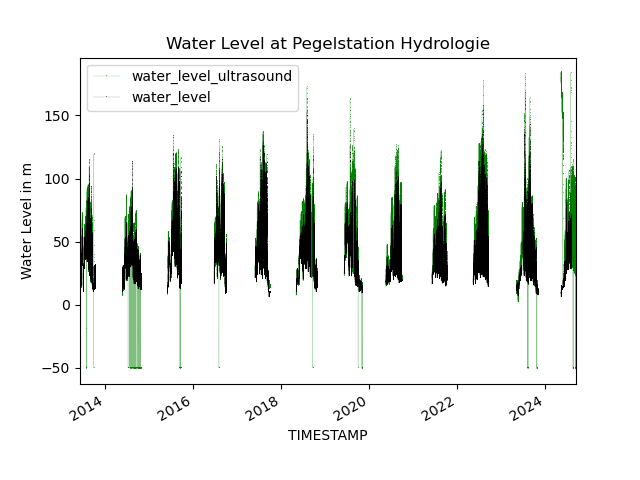
\includegraphics[width=0.49\textwidth]{plots_T/overview_water_level.png}
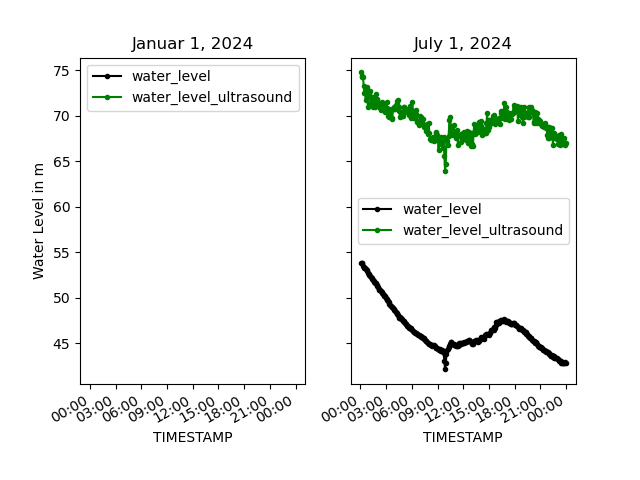
\includegraphics[width=0.49\textwidth]{plots_T/overview_water_level_2days.png}
\caption{Water Level}
\label{fig:water_level}
\end{figure}

\paragraph{Air Temperatures}
(See Figure \ref{fig:air_temperature}) The air temperature of Schwarzkögele is not available in the first 2 years and generally lower than the air temperatures at Pegelstation Meteorologie. This is due to the greater height of Schwarzkögele.
\begin{figure}[H]
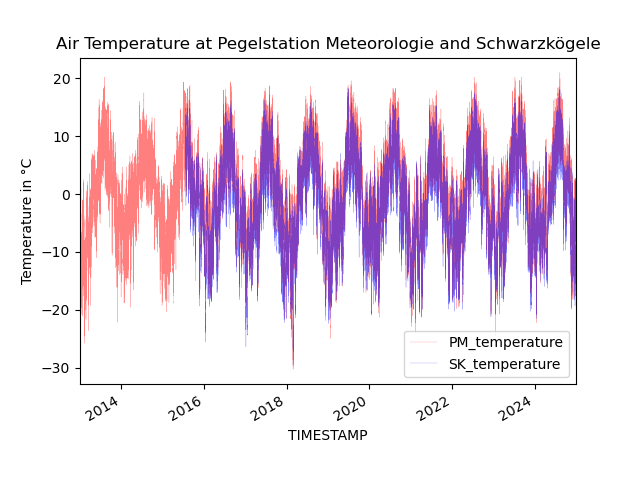
\includegraphics[width=0.49\textwidth]{plots_T/overview_temperature.png}
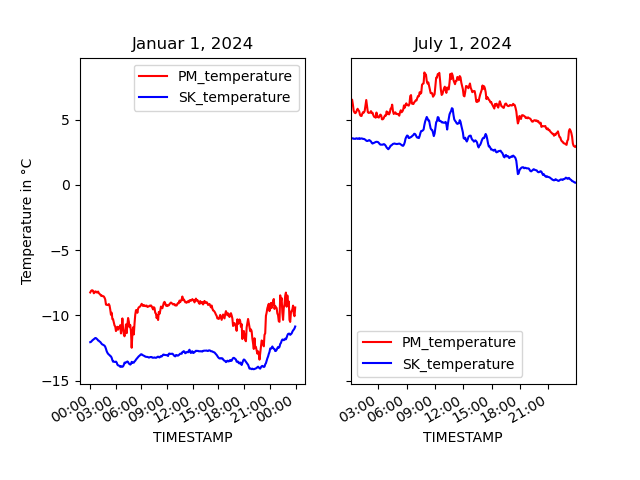
\includegraphics[width=0.49\textwidth]{plots_T/overview_temperature_2days.png}
\caption{Air Temperature}
\label{fig:air_temperature}
\end{figure}

\paragraph{Atmospheric Pressure} The atmospheric pressure at Pegelstation Meteorologie with values around 735~HPa reflects the height of the measurement station 2640~m compared to the mean sea level atmospheric pressure of 1013.25~HPa
(See Figure \ref{fig:atmospheric_pressure})
\begin{figure}[H]
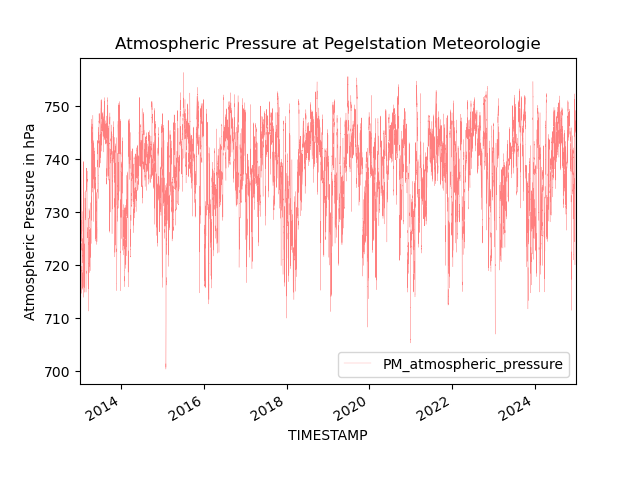
\includegraphics[width=0.49\textwidth]{plots_T/overview_pressure.png}
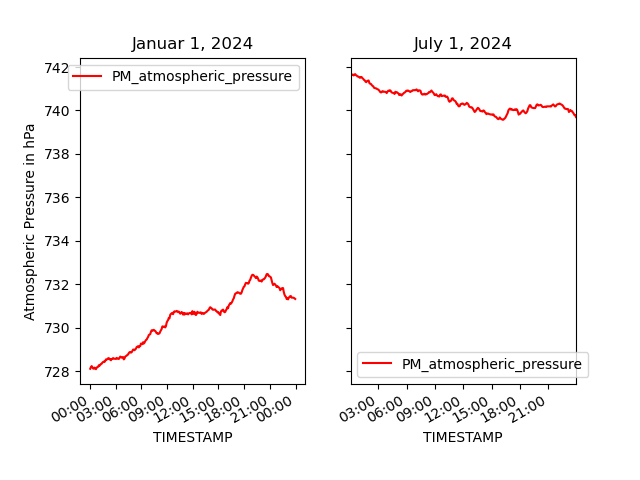
\includegraphics[width=0.49\textwidth]{plots_T/overview_pressure_2days.png}
\caption{Atmospheric Pressure}
\label{fig:atmospheric_pressure}
\end{figure}

\paragraph{Relative Humidity}
(See Figure \ref{fig:relative_humidity}) The plots for relative humidity show a great difference between the measurement stations Schwarzkögele and Pegelstation Meteorologie. As relative humidity should be in the range between 0 and 100 and SK\_relative\_humidity shows a different behavior from some time in 2018 SK\_relative\_humidity has to be regarded invalid and should not be used for modeling.
\begin{figure}[H]
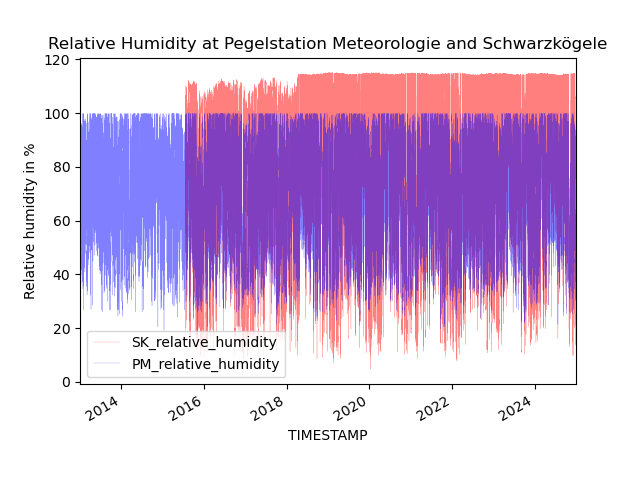
\includegraphics[width=0.49\textwidth]{plots_T/overview_humidity.png}
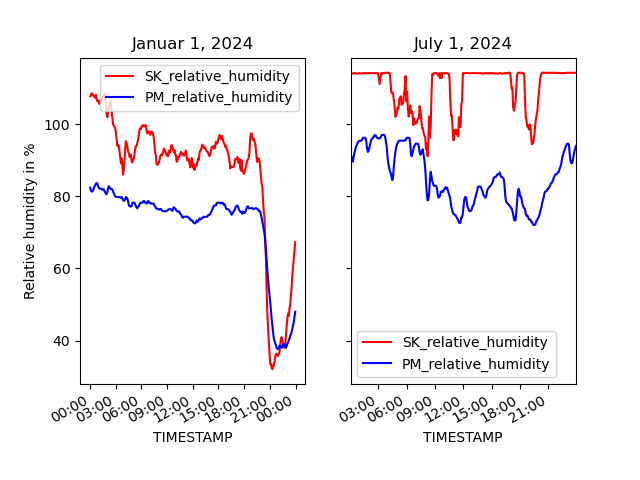
\includegraphics[width=0.49\textwidth]{plots_T/overview_humidity_2days.png}
\caption{Relative Humidity}
\label{fig:relative_humidity}
\end{figure}

\paragraph{Precipitation}
(See Figure \ref{fig:precipitation}) The precipitation PM\_precipitation measured in mm/(5 min) has measurement gaps during the winter in the earlier years because the measurement instrument was then disassembled in winter. The precipitation PM\_precipitation\_cum measured in mm is the cumulative precipitation during a year and is corrupted by the evaporation of water from the measurement instrument. PM\_precipitation\_cum shows a significant measurement gap in 2019. As the precipitation is measured in two ways it should be sufficient to keep one measurement.
\begin{figure}[H]
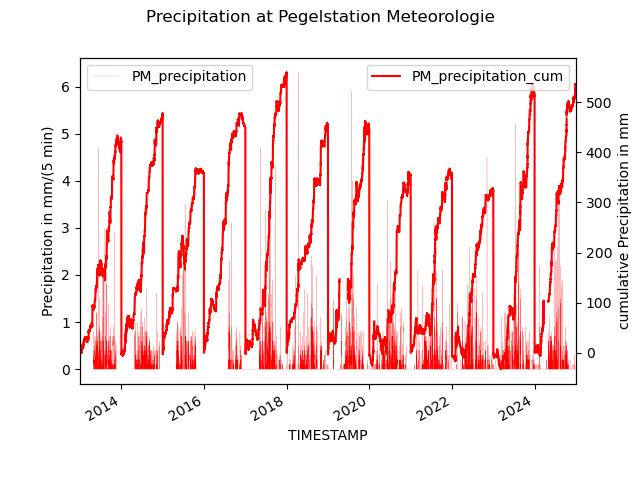
\includegraphics[width=0.49\textwidth]{plots_T/overview_precipitation.png}
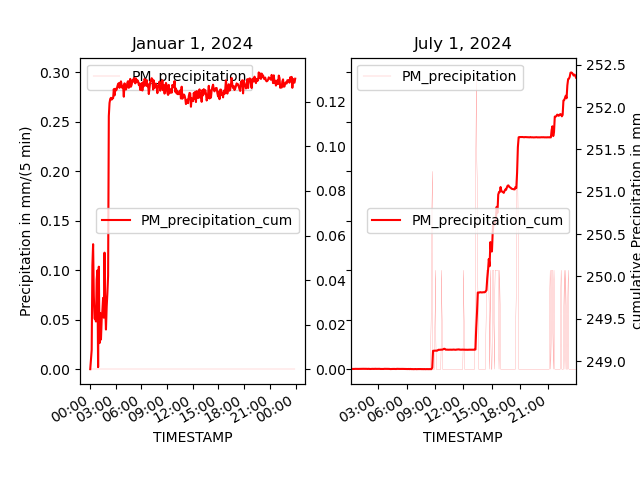
\includegraphics[width=0.49\textwidth]{plots_T/overview_precipitation_2days.png}
\caption{Precipitation}
\label{fig:precipitation}
\end{figure}

\paragraph{Snow Height}
(See Figure \ref{fig:snow_height}) The snow height exhibits several missing values. However as the snow height does not show larger variations over time it should be safe to interpolate missing values.
\begin{figure}[H]
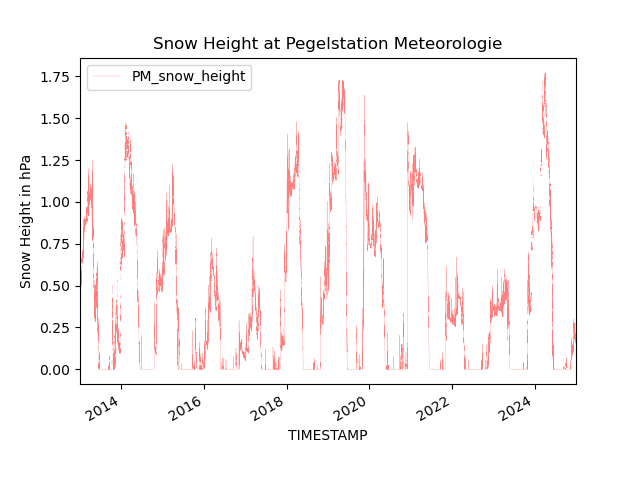
\includegraphics[width=0.49\textwidth]{plots_T/overview_snow.png}
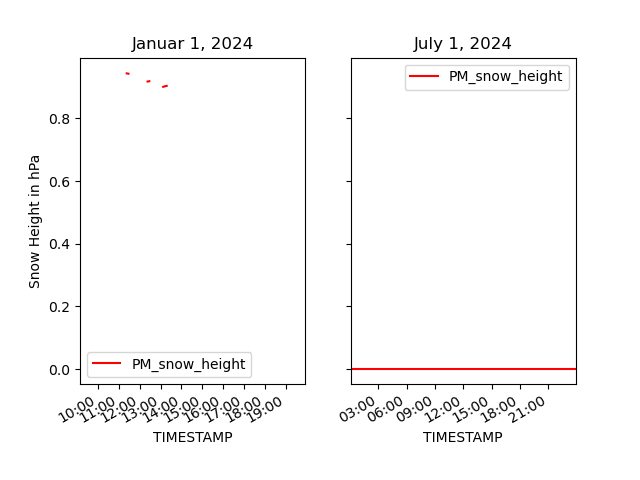
\includegraphics[width=0.49\textwidth]{plots_T/overview_snow_2days.png}
\caption{Snow Height}
\label{fig:snow_height}
\end{figure}

\paragraph{Wind Speed}
(See Figure \ref{fig:wind_speed}) The wind speeds measured at Pegelstation Meteorologie and Schwarzkögele show a little offset probably because of the use of different measurement instruments.
\begin{figure}[H]
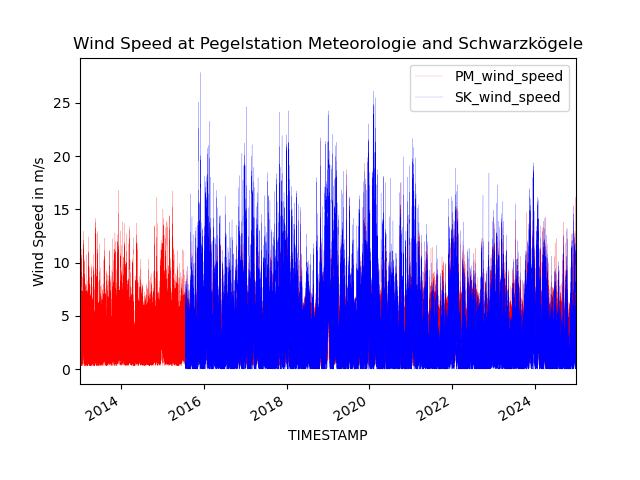
\includegraphics[width=0.49\textwidth]{plots_T/overview_wind_speed.png}
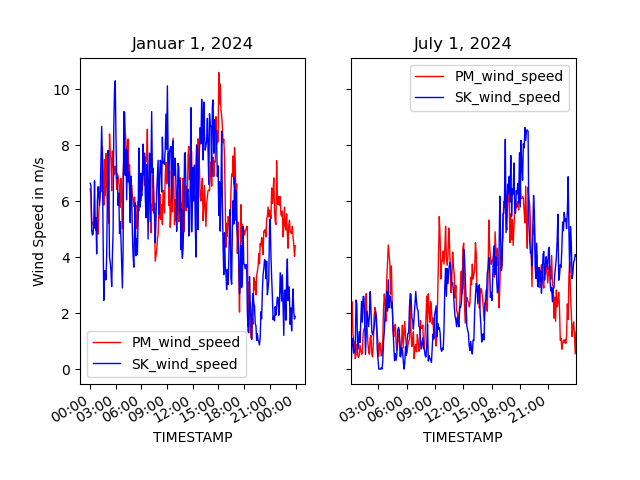
\includegraphics[width=0.49\textwidth]{plots_T/overview_wind_speed_2days.png}
\caption{Wind Speed}
\label{fig:wind_speed}
\end{figure}

\paragraph{Wind Direction}
(See Figure \ref{fig:wind_direction}) There are 2 main wind directions around 150 and 330 degrees at the measurement stations which are more pronounced at Pegelstation Meteorologie located deeper down the glacier valley. 
\begin{figure}[H]
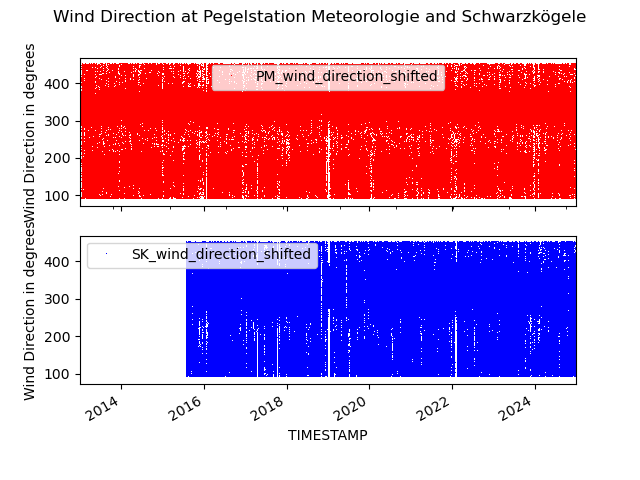
\includegraphics[width=0.49\textwidth]{plots_T/overview_wind_direction.png}
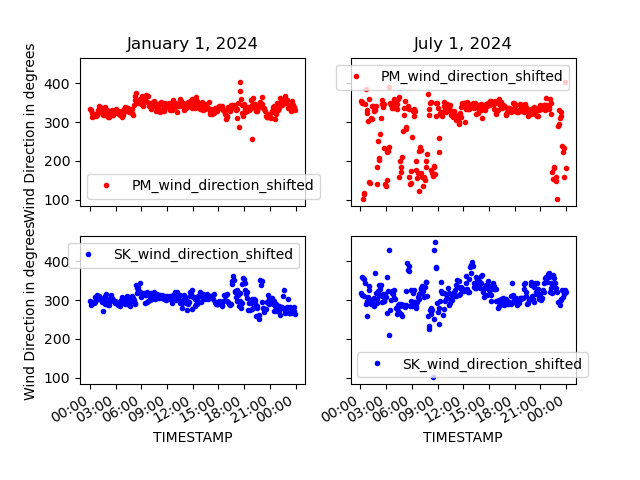
\includegraphics[width=0.49\textwidth]{plots_T/overview_wind_direction_2days.png}
\caption{Wind Direction}
\label{fig:wind_direction}
\end{figure}

\paragraph{Short Wave Radiation}
(See Figure \ref{fig:radiation})Two kinds of short wave radiation are measured at Pegelstation Meteorologie. The Short Wave Radiation Downward (PM\_SWD) is the short wave radiation coming from above mainly from the sun. It is strongest during the summer. The Short Wave Radiation Upward (PM\_SWU) is the short wave radiation coming from below. It is mainly part of the short wave radiation from above reflected by the ground. In winter a lot of the short wave radiation from the sun is reflected by snow on the ground but when the snow is gone the Short Wave Radiation Upward is levelling.
\begin{figure}[H]
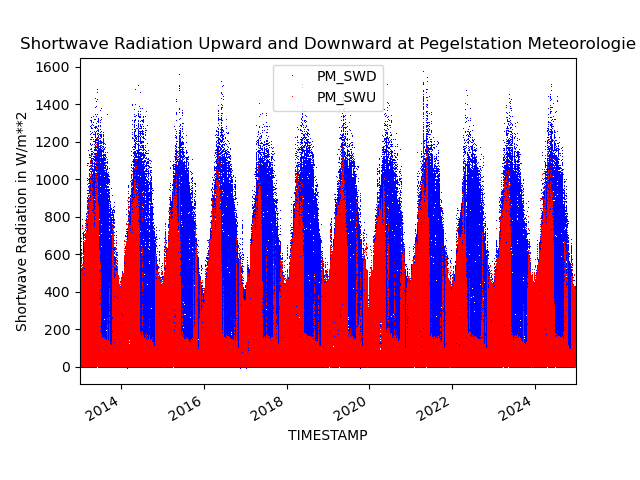
\includegraphics[width=0.49\textwidth]{plots_T/overview_radiation.png}
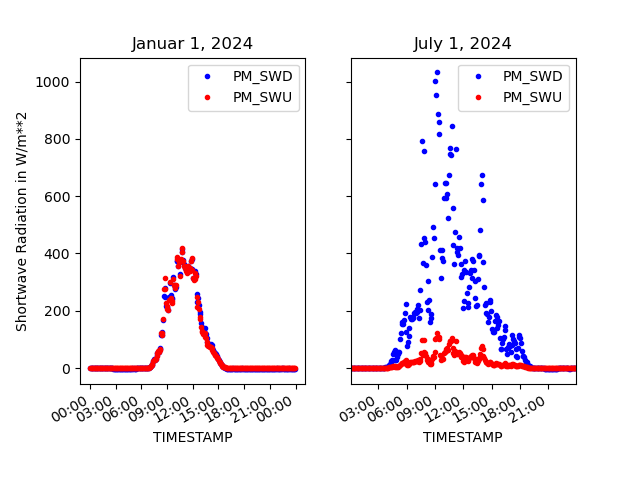
\includegraphics[width=0.49\textwidth]{plots_T/overview_radiation_2days}
\caption{Radiation}
\label{fig:radiation}
\end{figure}

\newpage
\section{Project Workflow / Summary}

To give an upfront information the following chapter shows how the workflow i.e. the data handling was carried out to generate the predictions for the water level.
\subsection*{Component Description}
\begin{itemize}
    \item \textbf{Data\_prep.py (Preprocessing)}
    \begin{itemize}
        \item \textbf{Input:} 1. sweep: Raw uncleaned dataset.\\ Next sweeps: modified data (mod\_meteohydrodata.csv)
        \item \textbf{Process:} Fill gaps with data from the past (shift(xD). Remaining gaps (smaller than ca. 6h) filled with ffill().
        \item \textbf{Output:} \texttt{mod\_meteohydrodata.csv}.
    \end{itemize}
    
    \item \textbf{Data\_analysis.py (Data Analysis)}
    \begin{itemize}
        \item \textbf{Input:} \texttt{mod\_meteohydrodata.csv}.
        \item \textbf{Process:} Exploratory Data Analysis (EDA), Var- and covariance for PM variables, Rolling covariance between water level and variables with hight covariance in matrix to identify Lag Variables, Seasonal Effects and Temperature trend analysis with significance test acc. to Kendall.
        \item \textbf{Output:} Correlation heatmap, Covariance plots, Time plots 
    \end{itemize}
    
    \item \textbf{Feature\_Eng.py (Feature Engineering)}
    \begin{itemize}
        \item \textbf{Input:} \texttt{mod\_meteohydrodata.csv}.
        \item \textbf{Process:} Encoding is not necessary because DF consist only of measurement data.
        \begin{itemize}
            \item Because of computing time requirements the data set is accumulated from 5 min time intervals to daily based time stamp.
            \item Generation of Lag Variables with input from EDA.
            \item Creation of seasonality variables with sinusoidal function for day and year. The yearly seasonality is divided in a constant leg for winter period (no change in water level) and a half sin wave for the summer period.
            \item The variable snow storage is implemented to picture the presence of snow and ice during summer (glacier definition).
        \end{itemize}
        \item \textbf{Output:} \texttt{mod\_feature\_meteohydrodata\_hourly.csv} (or split matrices).
    \end{itemize}
    
    \item \textbf{ML\_x.py (Machine Learning)}
    \begin{itemize}
        \item \textbf{Input:} \texttt{mod\_feature\_meteohydrodata\_hourly.csv}.
        \item \textbf{Process:} Following ML models / predictor were investigated:
        \begin{itemize}
            \item LinearRegression
            \item Autoregressive models: Prophet and SAMIRA
            \item LazyPredictor (depending on test period length two different ML models were best rated)
            \item GammaRegressor (long test period)
            \item Histogram-based Gradient Boosting Regressor (short test period)
        \end{itemize}
        \item \textbf{Output:} Comparison of RMSE and $R^2$ metrics.
    \end{itemize}
\end{itemize}

% --- Definition der TikZ-Styles für den Ablaufplan ---
\begin{figure}[H]
\centering
\resizebox{\textwidth}{!}{%
\tikzset{
    script/.style = {rectangle, rounded corners, minimum width=4cm, minimum height=1cm, text centered, draw=blue!70, fill=blue!5, font=\bfseries},
    file/.style = {rectangle, minimum width=4cm, text width=5.5cm, minimum height=0.8cm, text centered, draw=green!60!black, fill=green!5, font=\ttfamily\small},
    process/.style = {rectangle, minimum width=5cm, text width=6cm, minimum height=1cm, draw=gray, fill=gray!5, font=\small},
    arrow/.style = {thick,->,>=stealth}
}
\begin{tikzpicture}[node distance=1.8cm, auto]

% --- SCHRITT 1: Data_prep.py ---
\node (raw) [file] {Raw Dataset / preprocessed\_meteohydrodata 2026-05-26.csv};
\node (prep) [script, below=of raw, yshift=-0.3cm] {Data\_prep.py (Preprocessing)};
\node (prep_proc) [process, right=of prep, xshift=1.5cm] {Gaps filled with past data (shift) and remaining small gaps (<6h) via ffill().};
\node (csv1) [file, below=of prep, yshift=-0.3cm] {mod\_meteohydrodata.csv};

% --- SCHRITT 2: Data_analysis.py ---
\node (analysis) [script, below=of csv1, yshift=-0.3cm] {Data\_analysis.py (Analysis)};
\node (anal_proc) [process, right=of analysis, xshift=1.5cm] {EDA, Var/Covariance, Rolling covariance for Lag identification, Kendall Significance Test.};
\node (plots) [file, below=of analysis, yshift=-0.3cm] {Heatmaps, Covariance \& Time Plots};

% --- SCHRITT 3: Feature_Eng.py ---
\node (feat) [script, below=of plots, yshift=-0.3cm] {Feature\_Eng.py (Feature Eng.)};
\node (feat_proc) [process, right=of feat, xshift=1.5cm] {Resampling (5min $\rightarrow$ hourly), Lag generation, Sinusoidal seasonality (winter constant, summer half-wave), Snow storage.};
\node (csv2) [file, below=of feat, yshift=-0.3cm] {mod\_feature\_meteohydrodata \_hourly.csv};

% --- SCHRITT 4: ML_x.py ---
\node (ml) [script, below=of csv2, yshift=-0.3cm] {ML\_x.py (Machine Learning)};
\node (ml_proc) [process, right=of ml, xshift=1.5cm] {Evaluation of: LinearRegression, Prophet, SARIMAX, LazyPredictor, GammaRegressor, HistGradientBoosting.};
\node (metrics) [file, below=of ml, yshift=-0.3cm] {Comparison Matrix (RMSE, $R^2$)};

% --- Pfeile und Verbindungen zeichnen ---
\draw [arrow] (raw) -- (prep);
\draw [arrow] (prep) -- (csv1);
\draw [arrow] (prep) -- (prep_proc);
\draw [arrow] (csv1) -- (analysis);
\draw [arrow] (analysis) -- (plots);
\draw [arrow] (analysis) -- (anal_proc);

% Verbindung von csv1 links herum zu Feature_Eng.py
\draw [arrow] (csv1.west) -- ++(-1cm,0) |- (feat.west);
\draw [arrow] (feat) -- (csv2);
\draw [arrow] (feat) -- (feat_proc);
\draw [arrow] (csv2) -- (ml);
\draw [arrow] (ml) -- (metrics);
\draw [arrow] (ml) -- (ml_proc);

% --- Schleife für "Next Sweeps" auf der RECHTEN Seite ---
\draw [arrow, dashed, red!70!black] (csv1.east) -- ++(8.5cm,0) -- node[anchor=west, color=black, font=\small\bfseries, pos=0.4] {Next Sweeps} ++(0,3.3cm) -| (raw.east);

\end{tikzpicture}
} % Ende von resizebox
\caption{Systematic Data and Modeling Workflow for Water Level Prediction}
\label{fig:workflow_pipeline}
\end{figure}

\section{Data Preprocessing}
\subsection{Preprocessing of the water level (Target Variable)}
For short periods of missing values the missing values of water\_level are interpolated. Longer gaps of missing values of water\_level are filled by the values of water\_level\_ultrasound that are adjusted to fit the last and first values of non missing values of the water\_level.

\subsection{Timestamp Handling}
Convert timestamps to datetime format and sort chronologically.

\subsection{Missing Values}
For the descriptive variables the two methods:

\begin{itemize}
    \item Forward shifting
    \item Forward filling
\end{itemize}
Were applied.

\vspace{\baselineskip}

For Temperature, Atmospheric pressure, Humidity, Wind speed, Wind direction and Solar radiation, missing values, which time period was within O(one day), were filled by data from one or two days before the data gap (Forward shifting).
The assumption is that the variables do not change significantly in the considered time interval. 
This approach is described in the following pictures.

\begin{figure}[H]
    \centering
    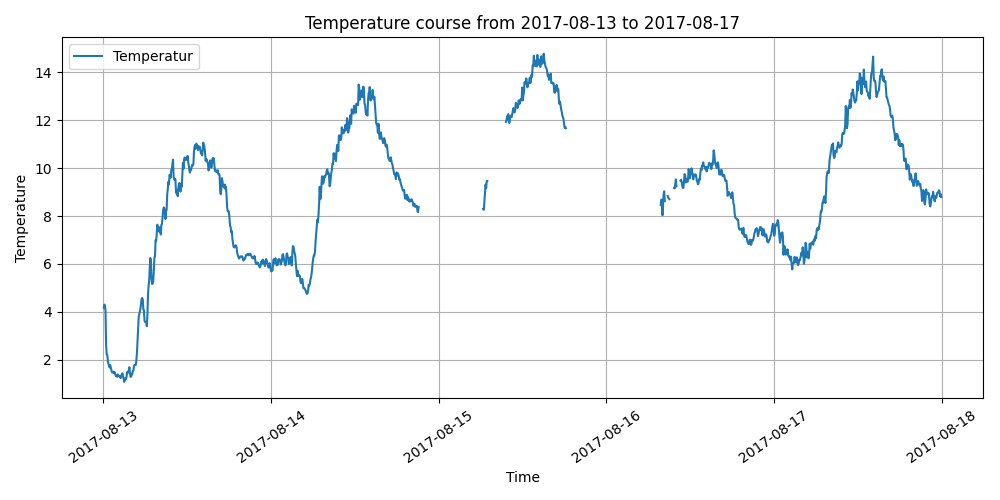
\includegraphics[width=\linewidth]{plots_H/Temp_cutout_raw.png}
    \caption{Temperature cutout with gap}
\end{figure}

The picture shows the raw data distribution of the temperature in the time interval 2017-08-13 to 2017-08-17 with gaps in the temperature course. The biggest gap is from 2017-08-15 18:17:30+00:00 to 2017-08-16 06:42:30+00:00, which was determined by a python script counting nan to find the biggest gaps. 

\begin{figure}[H]
    \centering
    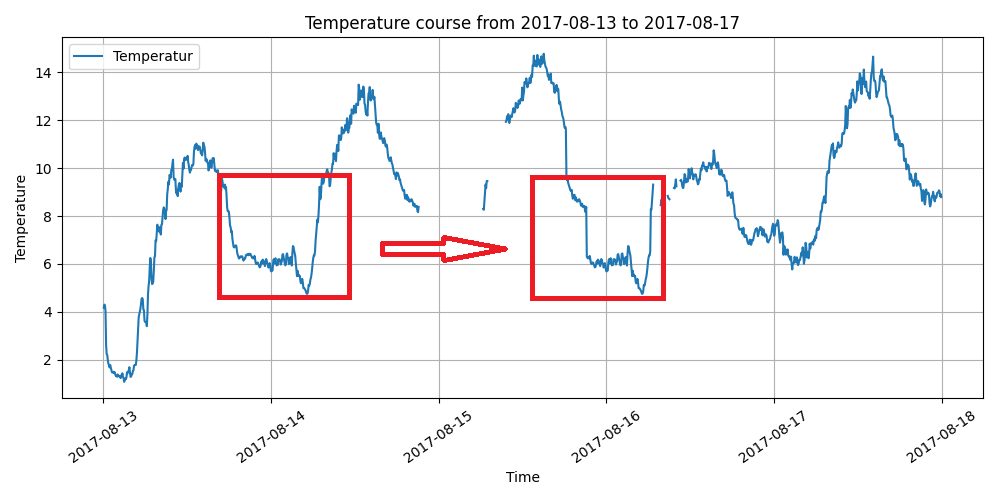
\includegraphics[width=\textwidth]{plots_H/Temp_cutout_mod_exp.png}
    \caption{Temperature cutout with closed gap}
\end{figure}

Like the above figure shows leads this method to discontinuities at the points where the data is connected (current / history data). With the above assumption the expectation is that this jump is in a tolerable range (e.g. dT < 5~K, dP < 1~HPa).
For the above example the jump of the temperature is 0.9°C over 2h.

The remaining gaps were filled by forward filling. Final result see picture below.

\begin{figure}[H]
    \centering
    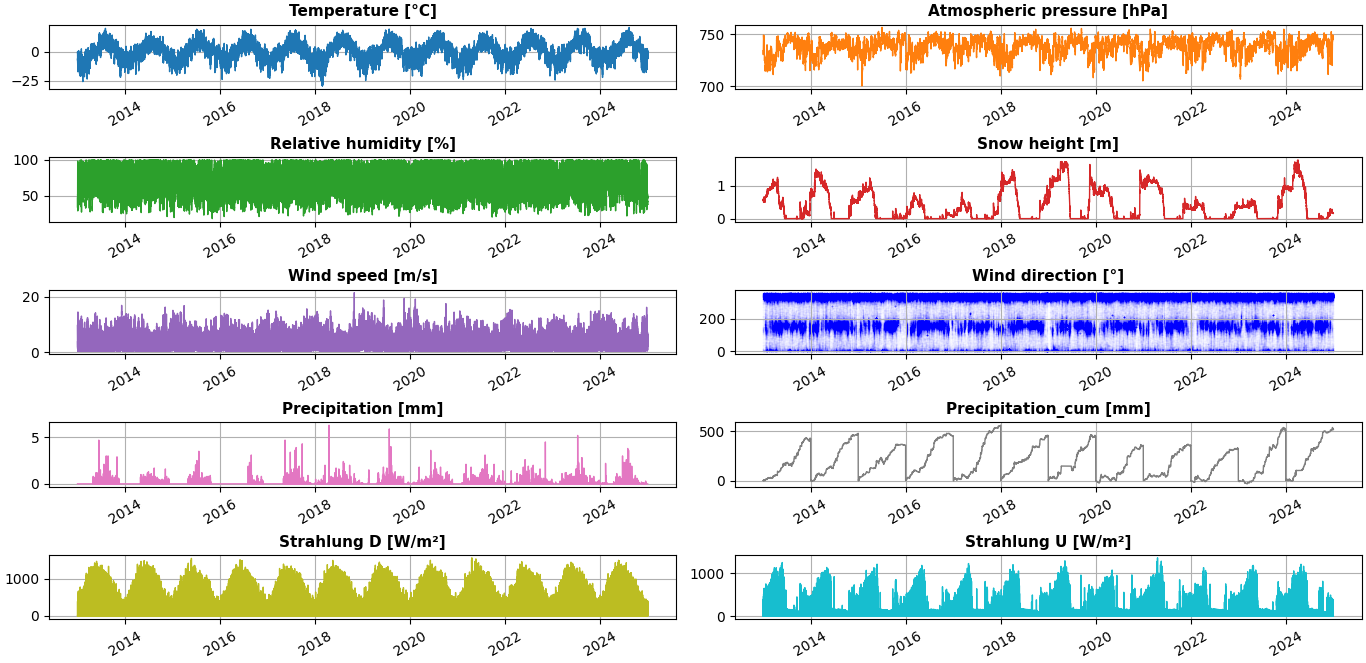
\includegraphics[width=\textwidth]{plots_H/Variab_PM_pre_processed.png}
    \caption{Explanatory Variables}
\end{figure}

The preprocessed water level is shown in the next picture.

\begin{figure}[H]
    \centering
    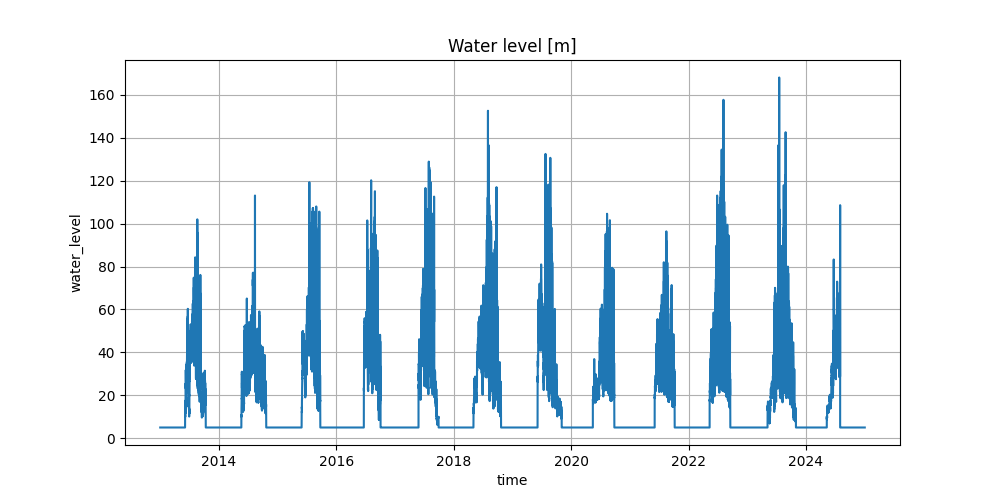
\includegraphics[width=\linewidth]{plots_H/Pre_pro_water_level.png}
    \caption{Preprocessed water level}
\end{figure}

\newpage
\subsection{Data Quality Checks}

Perform plausibility checks:

\begin{itemize}
    \item Negative precipitation values not seen
    \item Unrealistic sensor jumps not detected
\end{itemize}
These issues are not detected, see table Data Audit and the flollowing figure.

The variation in the values is due to physical factors, such as actual temperature fluctuations at the measurement site. A time-stable fluctuation should be observable over the measurement time period. The magnitude of the variations depends on the specific measurement variable, see figure below.
The variation in the differences between consecutive measurement values should remain within the range of the raw (unmodified) data.
The expected value of the measurement differences should be reasonable for 5 min steps and  within the limits of the measurement chains' accuracy. 

\begin{figure}[H]
    \centering
    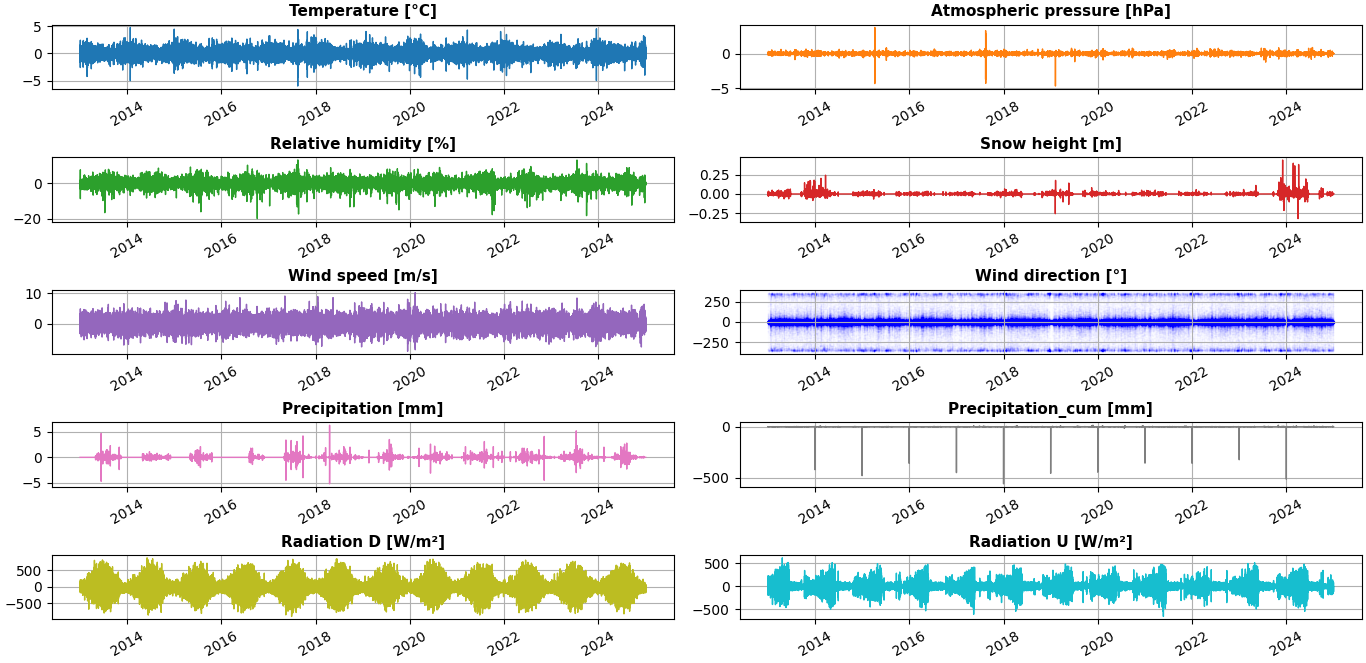
\includegraphics[width=\linewidth]{plots_H/diff_variab_PM.png}
    \caption{Explanatory Variables with difference, lag = 1 measurement}
\end{figure}

%-------------------------------------------------------
\newpage
\section{Exploratory Data Analysis}

\subsection{Correlation Analysis}

Initial correlations between variables investigated using correlation matrices (Pearson).

\begin{figure}[H]
    \centering
    \begin{adjustwidth}{-2cm}{-1.5cm} % Erlaubt dem Bild, 1.5cm links und rechts in den Rand zu ragen
        \centering
        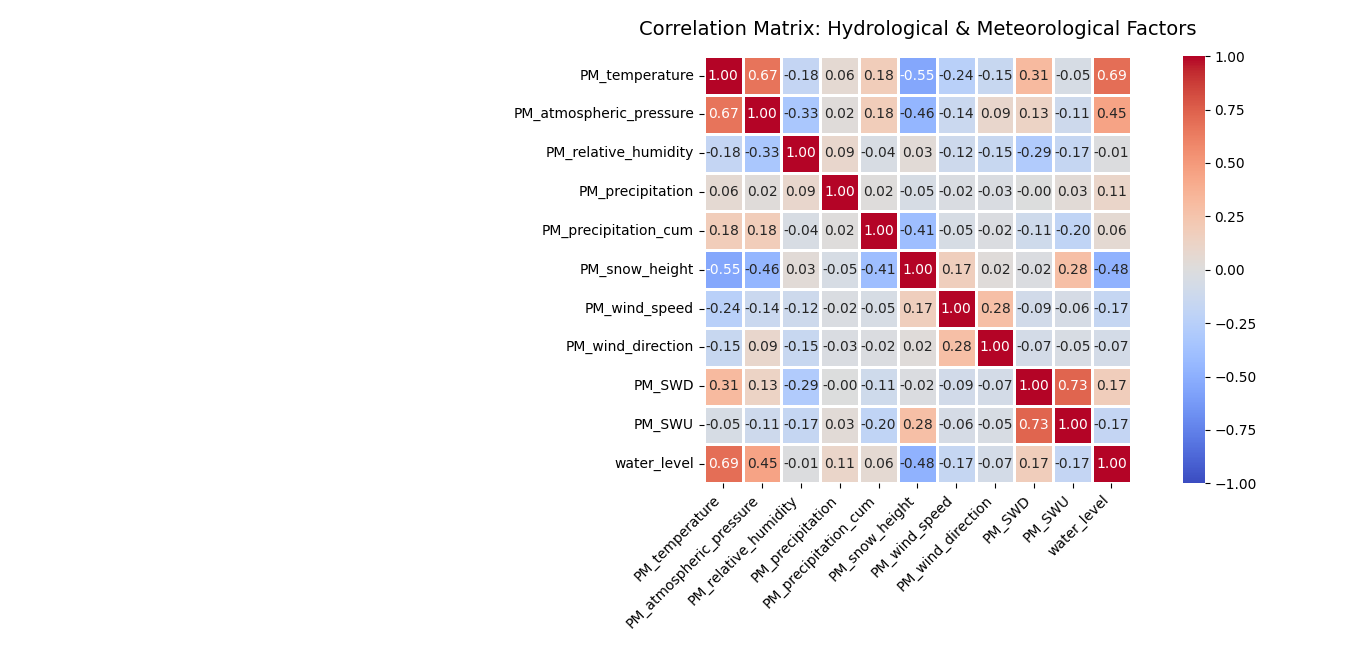
\includegraphics[width=\linewidth]{plots_H/Corr_matrix.png}
        \caption{Correlation between all Variables}
    \end{adjustwidth}
\end{figure}

Based on (0.1 = weak, 0.3 = moderate, 0.5 = strong) from the statistician  Jacob Cohen: Cohen, J. (1988). Statistical Power Analysis for the Behavioral Sciences (2nd ed.). Lawrence Erlbaum Associates, it can be seen that 3 variables have a strong influence (Temperature, Atmospheric pressure and Snow height.
Wind speed, Percipitation and Radiation have a weak influence.

However, simple correlations may not fully capture delayed hydrological responses.

\subsection{Lag Analysis with rolling covariance analysis}

Investigate delayed effects between weak predictors and the target variable.\\
The covariance analysis is determent with a time shift of 5 min. for a daily period.\\
This leads to an insight if there is a lag between explanatory variable and the water level.

\subsubsection{Temperature}

\begin{figure}[H]
    \centering
    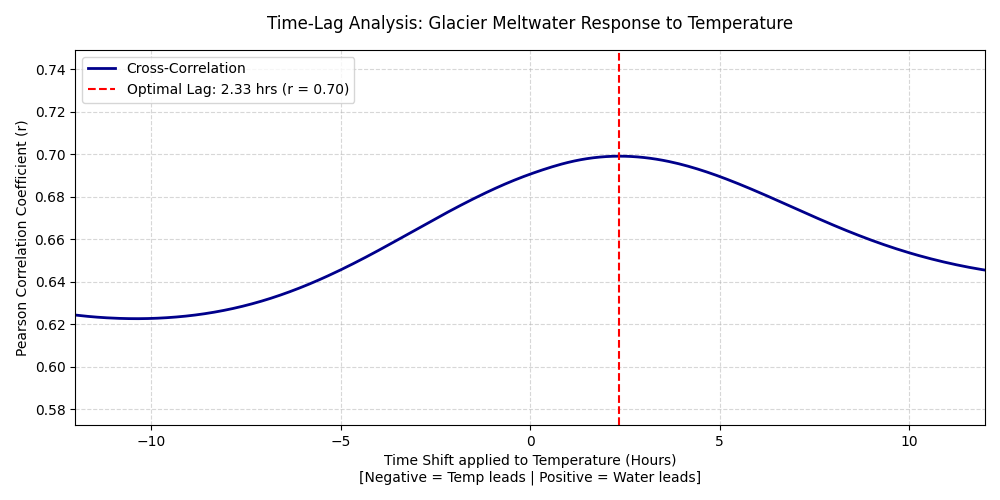
\includegraphics[width=0.9\linewidth]{plots_H/time_lag_wat_lev_temp.png}
    \caption{Time lag Temperature / Water level}
\end{figure}

The analysis shows an offset of 2,3 hours between temperature and water level.

\subsubsection{Atmospheric pressure, Radiation, Wind speed, Precipitation and Snow height}
Investigate delayed effects between weak predictors (Wind speed, Precipitation and Radiation) and the target variable.

\begin{figure}[H]
        \centering
        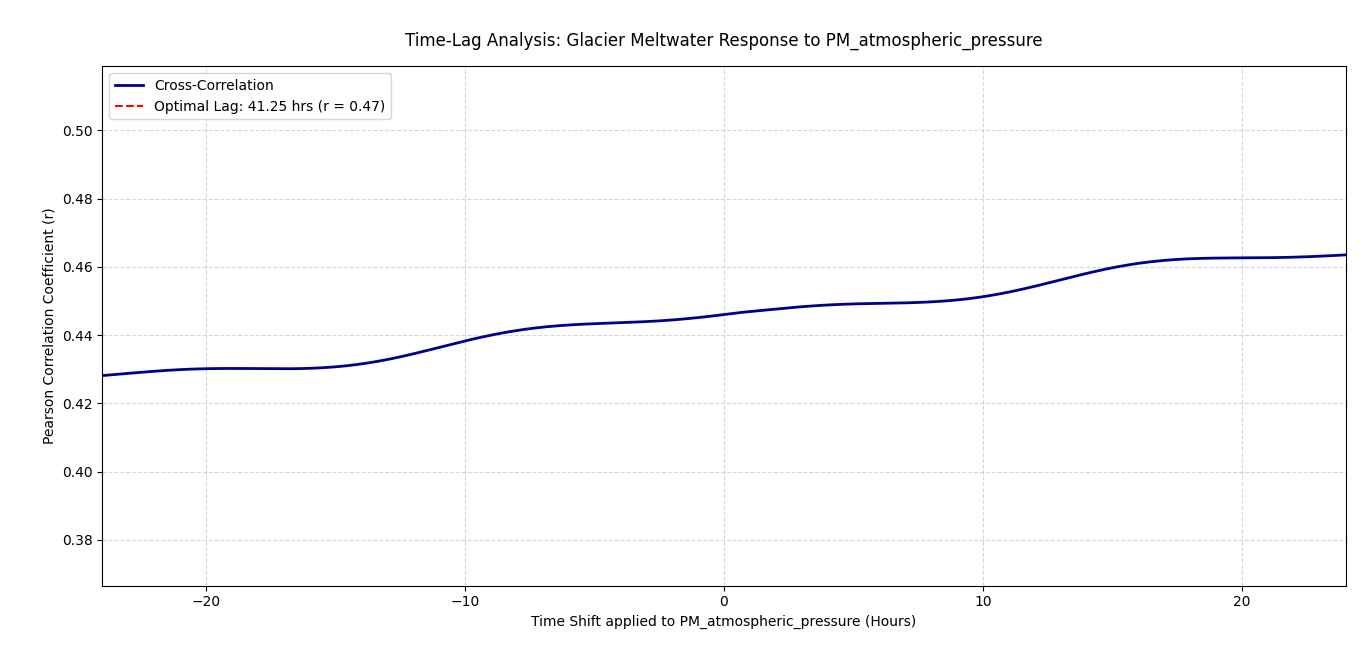
\includegraphics[width=\linewidth]{plots_H/time_lag_wat_lev_at_pres.png}
        \caption{Time lag Atmospheric pressure / Water level}
\end{figure}

The Atmospheric pressure is an indirect parameter, because there is no direct physical influence on the water level. The indirect influence is due to less clouds at high pressure, this is there is an effect on the radiation.

\begin{figure}[H]
        \centering
        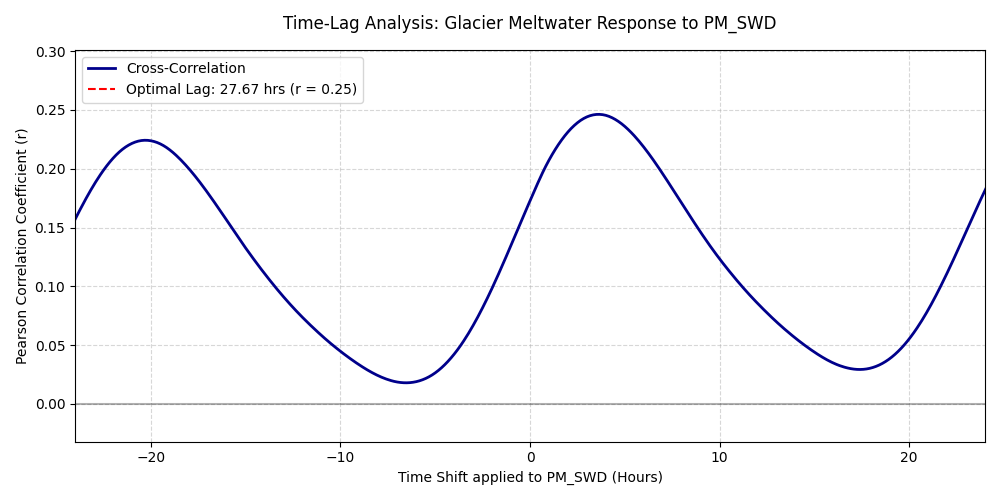
\includegraphics[width=\linewidth]{plots_H/time_lag_wat_lev_SWD.png}
        \caption{Time lag Radiation down/ Water level}
\end{figure}

Considering the time lag, the r value for the variable SWDown increases to 0.25. Which changes the influence from weak to moderate.

\begin{figure}[H]
        \centering
        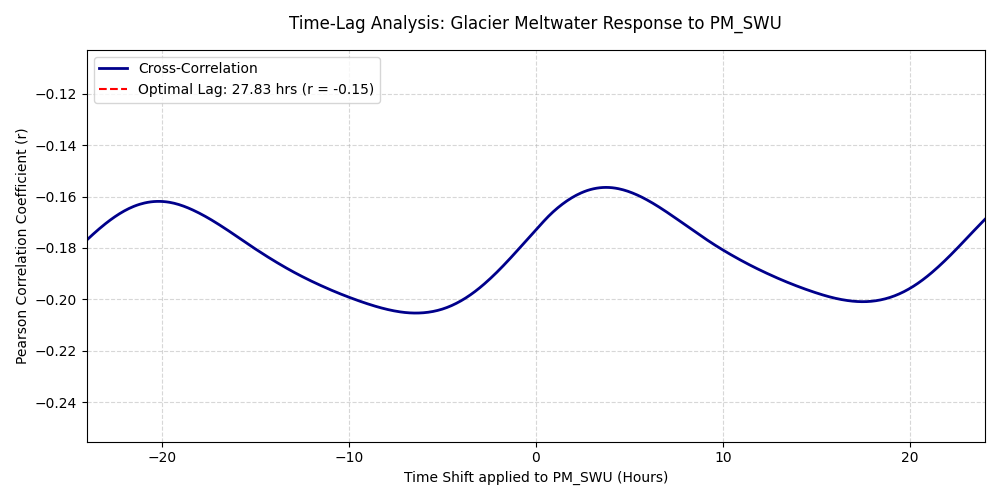
\includegraphics[width=0.9\linewidth]{plots_H/time_lag_wat_lev_SWU.png}
        \caption{Time lag Radiation up/ Water level}
\end{figure}

The time lag analysis shows nearly no change of the value SWU(p), this is the influence is still weak.

This behavior is physically cohered. Because due to the SWU radiation the snow lose energy (makes it cooler), due to the SWD radiation it gathers energy(makes it warmer). This is SWD generates potentially drain.

The snow height could have an offset because of the glacier structure (caves or other capacities for storing).

\begin{figure}[H]
        \centering
        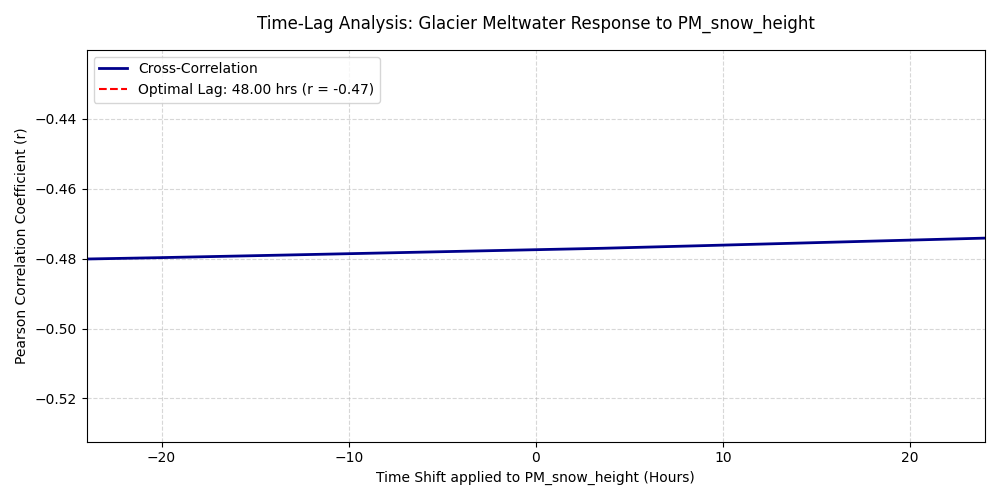
\includegraphics[width=0.9\linewidth]{plots_H/time_lag_wat_lev_snow.png}
        \caption{Time lag Snow height / Water level}
\end{figure}

There is nearly no offset between snow melting and water level.
What is reasonable when no capacities present.

\newpage
\subsection{Seasonal Effects}

At first the seasonal effects and trends for the target variable are considered.

\begin{figure}[H]
        \centering
        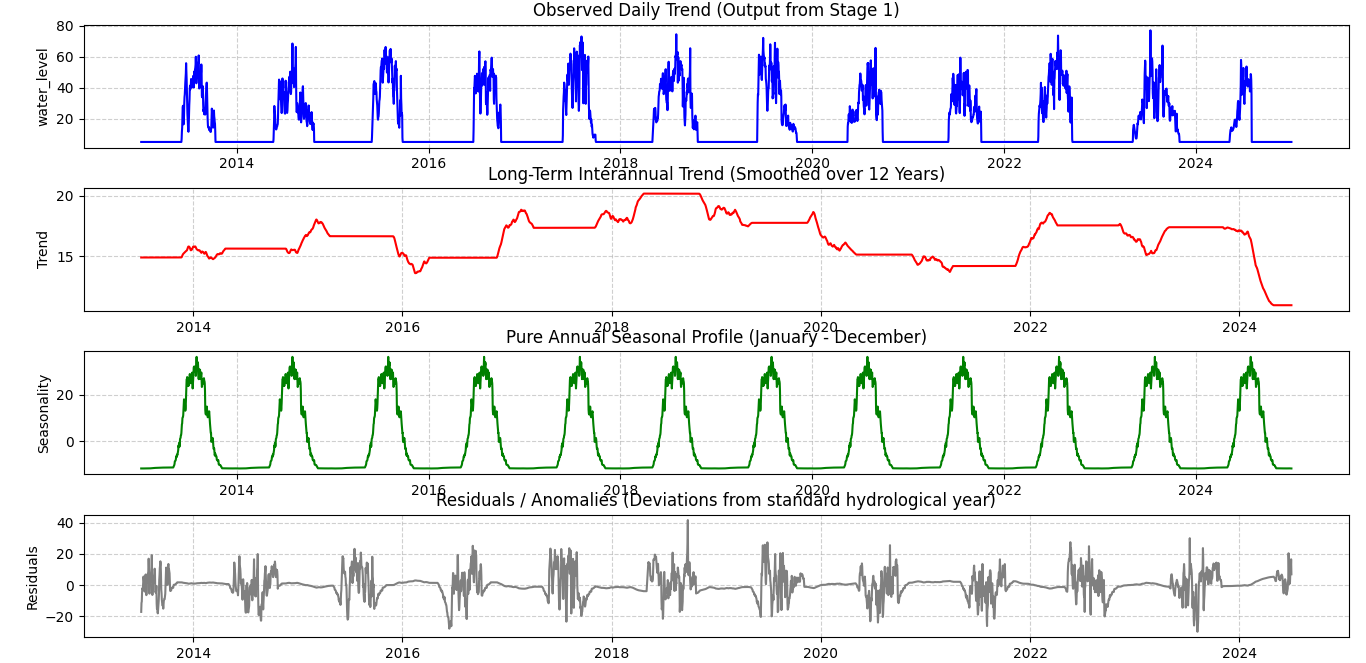
\includegraphics[width=0.9\linewidth]{plots_H/deco_season_WL.png}
        \caption{Water level}
\end{figure}
The trend shows a maximum of the water level in the year 2019.
The seasonal effects represent the four seasons of a year.

The most correlated variable temperature is next decomposed.

\begin{figure}[H]
        \centering
        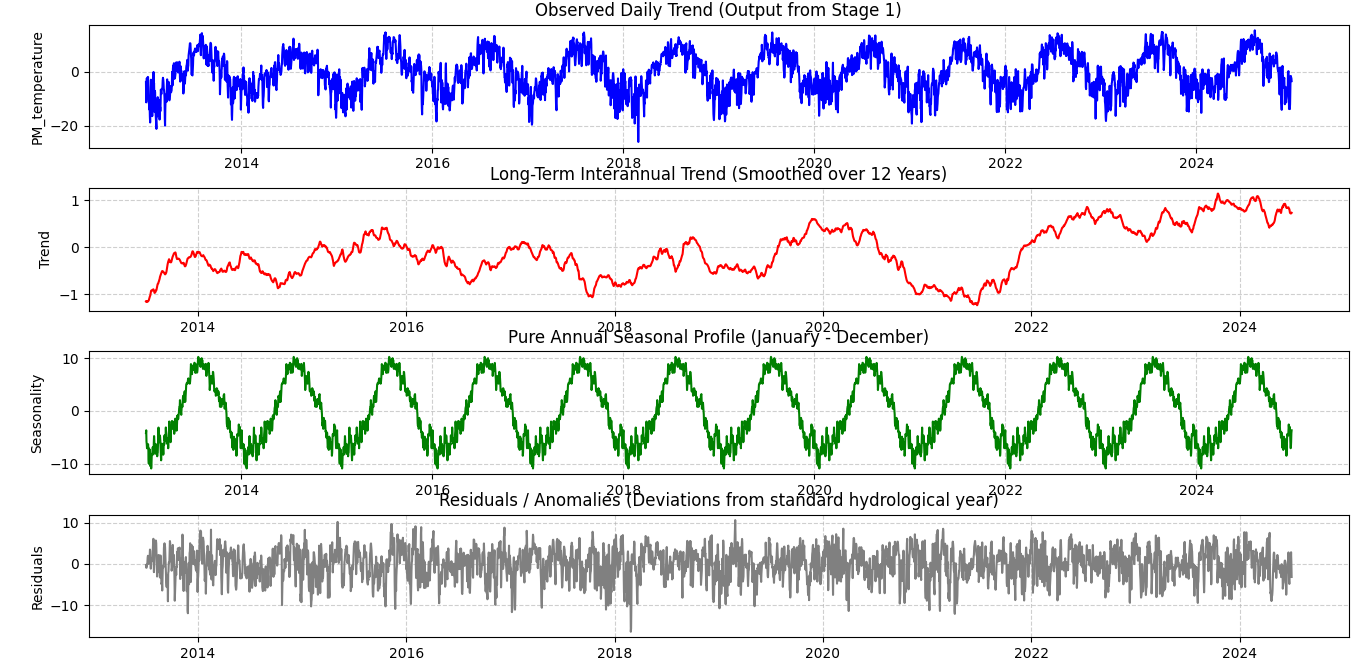
\includegraphics[width=\linewidth]{plots_H/deco_season_PM_temp.png}
        \caption{Temperature}
\end{figure}

The trend shows an increase over time with around 1°C.
The seasonality follows the seasons of the year.

\begin{figure}[H]
            \centering
            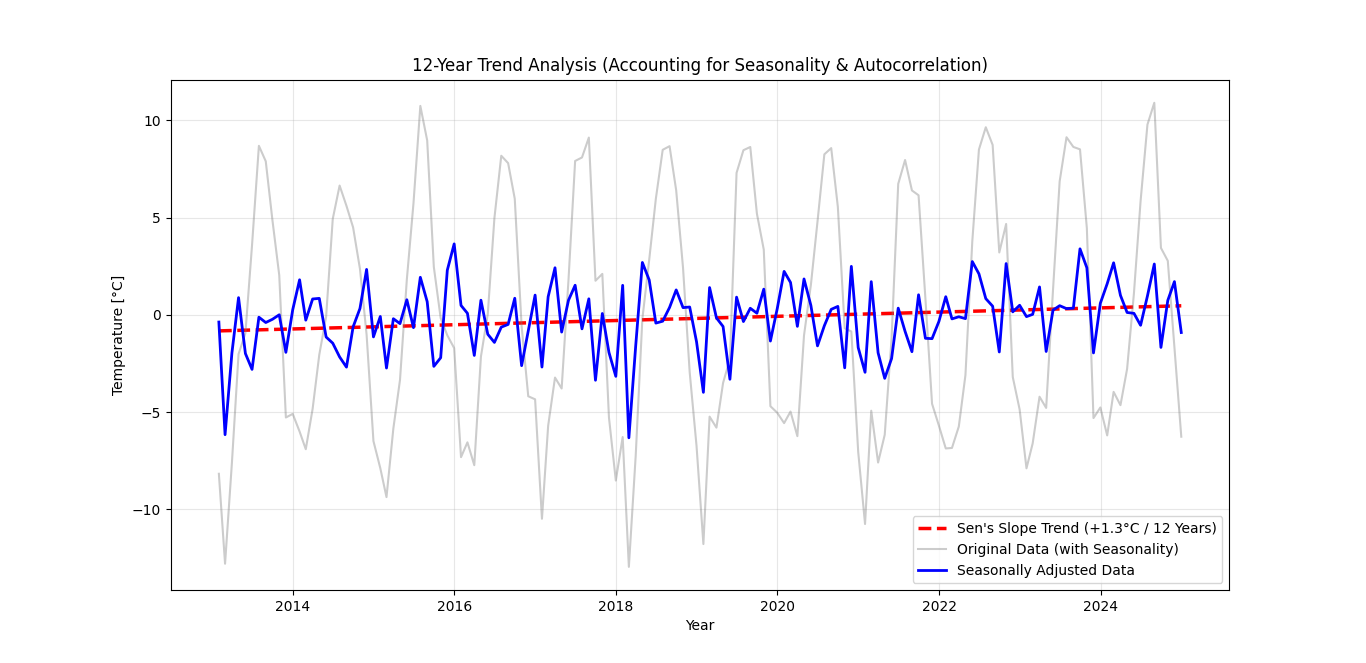
\includegraphics[width=\linewidth]{plots_H/Temperature_Trend.png}
            \caption{Temperature trend analysis}
\end{figure}

To identify a scientifically valid long-term trend from the 1.2 million raw temperature data points (PM\_temperature), the following three-step statistical workflow was applied:Monthly Aggregation: The high-resolution raw data was resampled to monthly mean values (.resample('ME')). This reduced noise and compressed the dataset into exactly 144 consistent data points over the 12-year period.Seasonal Decomposition: An additive seasonal decomposition was performed to isolate the sharp summer-to-winter fluctuations (seasonality). Subtracting this seasonal component yielded the Seasonally Adjusted Data (the baseline trend free from yearly weather cycles).Autocorrelation-Corrected Trend Test: A Correlated Seasonal Mann-Kendall Test was applied to the adjusted series. This specific test accounts for serial dependency (autocorrelation)—the tendency of consecutive months to influence one another. Mathematically, it adjusts (inflates) the variance of the test statistic to ensure that short-term weather phases do not fake a long-term climate trend, see fig. 24.

\begin{figure}[H]
            \centering
            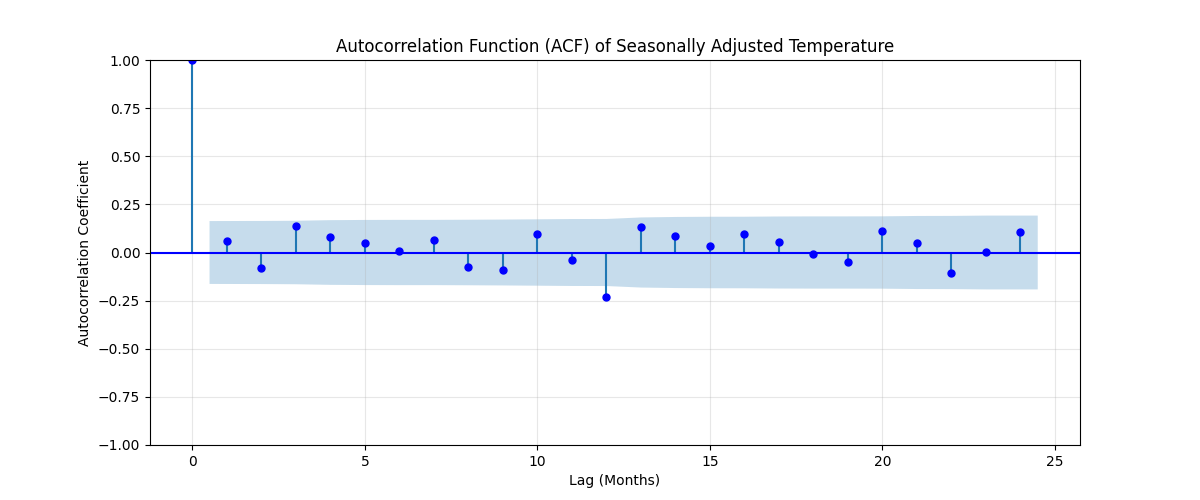
\includegraphics[width=\linewidth]{plots_H/ACF_Temperature.png}
            \caption{Temperature trend analysis}
\end{figure}

Trend Quantification: Sen's Slope was calculated within the test framework to determine the true magnitude of the change. This confirmed a steady, statistically robust temperature increase of approximately 1.3 °C over the entire 12-year period.

\begin{table}[H]
    \centering
    \caption{Climate Trend Significance Report (International Standards)}
    \label{tab:climate_trend_report}
    \begin{tabular}{ll}
        \toprule
        \textbf{Metric / Parameter} & \textbf{Value / Analysis Result} \\
        \midrule
        Analysis Period & 2013-01-01 to 2024-12-31 \\
        Total Observations & 144 months (Aggregated from 5-min data) \\
        Trend Direction & \textbf{INCREASING} \\
        $P$-Value ($p$) & $0.035440$ \\
        Statistical Status & \textbf{SIGNIFICANT} ($\alpha < 0.05$) \\
        Calculated Slope & 0.1135\,\textdegree C per year \\
        Extrapolated Change & \textbf{+1.36\,\textdegree C} over the 12-year period \\
        \midrule
        \multicolumn{2}{l}{\textbf{Methodological References for Reporting:}} \\
        \multicolumn{2}{l}{\small -- Trend Significance: Seasonal Kendall Test (Hirsch et al., 1982)} \\
        \multicolumn{2}{l}{\small -- Slope Robustness: Seasonal Sen's Slope Estimator (Gilbert, 1987)} \\
        \bottomrule
    \end{tabular}
\end{table}

\newpage
\section{Feature Engineering}

\subsection{Feature Engineering for Machine Learning Models}

\subsubsection{Time averaging}

The data is aggregated from a 5min frequency to a daily based data set. \\
Result df\_daily.

\subsubsection{Lag Feature}

\paragraph{Water Level}
The water level depends on the water level in the past.
To implement that a lag feature for the water level is generated with one day lag. \\
Result \texttt{df\_daily['wl\_lag1d']}
PROBLEM: If it is done in this way, a data leakage is generated for the variable, which should be predicted.\\
Lead to excellent results, but as the water level for the future is not known, these lag variable can not been calculated for the prediction period.\\

\paragraph{Temperature, SWD, Wind Speed and Precipitation}
According to the Data Analysis the moving covariance analysis (dt =5min) for the temperature and the water level shows a maximum at a time shift of ca. 2,3h. \\
This is two lag variables are generated with a time shift of two hours respectively with three hours.\\
The same is for the other variables (SWD,Wind Speed and Precipitation) with different time shifts for their maximum.

\subsubsection{Snow Memory}
The snow height measurement stagnates in the spring to fall season.
There is still snow and ice on the glacier (that makes a glacier).
To estimate this condition the variable snow storage is generated.
It takes the last snowfall height as a capacity with is reduced over the year when the temperature on the PM station is above zero degree Celsius.\\
storage = storage - melted snow.
melted snow = K  x Tmax , Tmax > 0 or zero.

\subsubsection{Cyclic yearly feature}

According to the Data Analysis a yearly seasonality was implemented with a maximum in summer and a constant value between October and April.\\
The maximum in the summer is continuously generated with a sin-function.
Result \texttt{df\_daily['summer\_wave']}

\subsection{Feature Engineering for Deep Learning Models}

The input for Deep Learning Models has to be different from the input for Machine Learning Models because of the different nature of Machine Learning Models and Deep Learning Models especially under the circumstances of time series data. Machine Learning Models can produce outputs independent of the length of the input (the length of the time series). Simple Deep Learning Models always take inputs of the same size and return outputs of the same size. This applies also to the length of the time series given that the Deep Learning Model is to output a result dependent on the time of the input time series. The use of a Deep Learning Model is said to catch non-linear relationships in the data so there is no need to set up features regarding time lags. As Deep Learning Models are said to be prone for problems with discontinuous data a variable with an yearly artificial discontinuity is feature-engineered. Having stated this it will follow the feature engineering comprising the creation of a new time variable, the conversion of the wind variables (PM\_wind\_speed, PM\_wind\_direction, SK\_wind\_speed, SK\_wind\_direction), the conversion of the cumulative precipitation PM\_precipitation\_cum and the deletion of some variables

\paragraph{Creation of a new time variable}
During the set up of the input data for a first Deep Learning Model it was a problem that the data loses track of time and there was no way to create a complete time series from the output of the Deep Learning Model. Therefore a new linear variable time\_s\_norm is created that is the time in seconds since 2013-01-01 00:00:00 normalized to be 0 at 2013-01-01 00:02:30 and 1 at 2024-12-31 23:57:30.

\paragraph{Conversion of the wind variables}
The wind direction in degrees is very variable and quite often there is a jump from just below 360 degrees to just above 0 degrees. By converting PM\_wind\_speed and PM\_wind\_direction (SK\_wind\_speed and SK\_wind\_direction) to a wind vector\\PM\_wind\_speed\_X\_direction and PM\_wind\_speed\_Y\_direction\\(SK\_wind\_speed\_X\_direction and SK\_wind\_speed\_Y\_direction)\\this effect can be eliminated.

\paragraph{Conversion of the cumulative precipitation}
The cumulative precipitation PM\_precipitation\_cum measured shows a yearly discontinuity at the beginning of the year because of the reset of the measurement data of the cumulative precipition to zero. It is not just a measurement of the precipitation but also the evaporation of water from the measurement instrument. Therefore two new variables are created by first taking the difference between each measurement value and the value one time step before this measurement value and then storing the positive values in a variable precipitation and the negative values in a variable evaporation.

\paragraph{Deletion of variables}
The variable SK\_relative\_humidity is deleted because of obvious malfunctioning of the measurement instrument during the whole measurement period. The variable PM\_precipitation has pronounced measurement gaps in the beginning of the whole measurement period and measures about the same as PM\_precipitation\_cum and is therefore deleted. The variable water\_level\_ultrasound is deleted because it just served to fill the gaps of water\_level.

After the splitting in a training dataset, a validation dataset and a test dataset all variables except the new time variable time\_s\_norm and the target variable water\_level are standardized by removing the mean of the training dataset and scaling to the unit variance of the training dataset.

\newpage
\section{Model Application}

\subsection{Model Application of Machine Learning Models}

For all models the train / test split were done explicit by fix dates.
After the split the "StandardScaler()" were used. Fitted with the train data and applied to the test data.
The performances of the models were checked by RMSE and the Coefficient of determination.

Start with simple and interpretable model.

\subsubsection{Linear Regression}

This provides a reference performance level.
First approach with plain data set, i.e. without implementation of features from the feature engineering (FE) step.

Only data from the Pegelstation Meteorologie (PM) were considered.

Second approach, the features from FE analysis were implemented step by step to evaluate the influence on the model.

\begin{itemize}
    \item Day and yearly seasonality (via sinusoidal functions)
    \item Lag features (Temperature, Radiation, Wind speed, Precipitation)
    \item Snow storage
\end{itemize}

\paragraph{Results}

\begin{figure}[H]
    \centering
    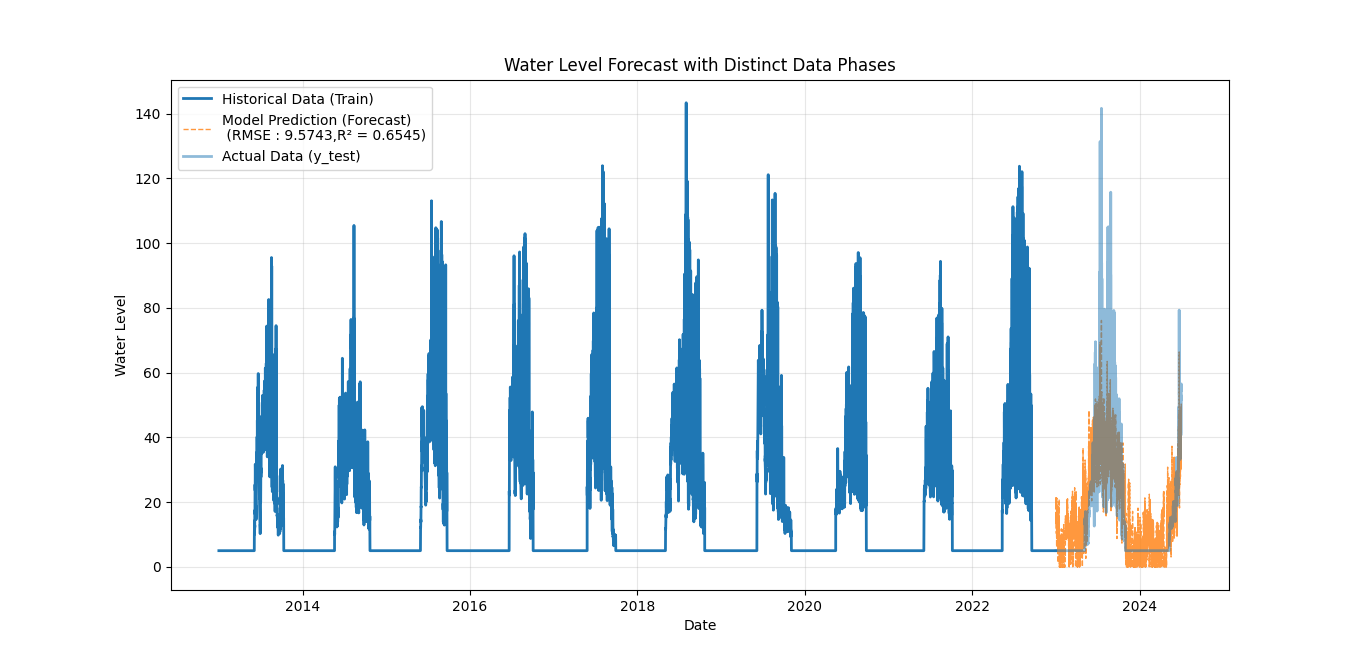
\includegraphics[width=\linewidth]{plots_H/WL_FE_plain.png}
    \caption{Water level, plain data}
\end{figure}

\begin{figure}[H]
    \centering
    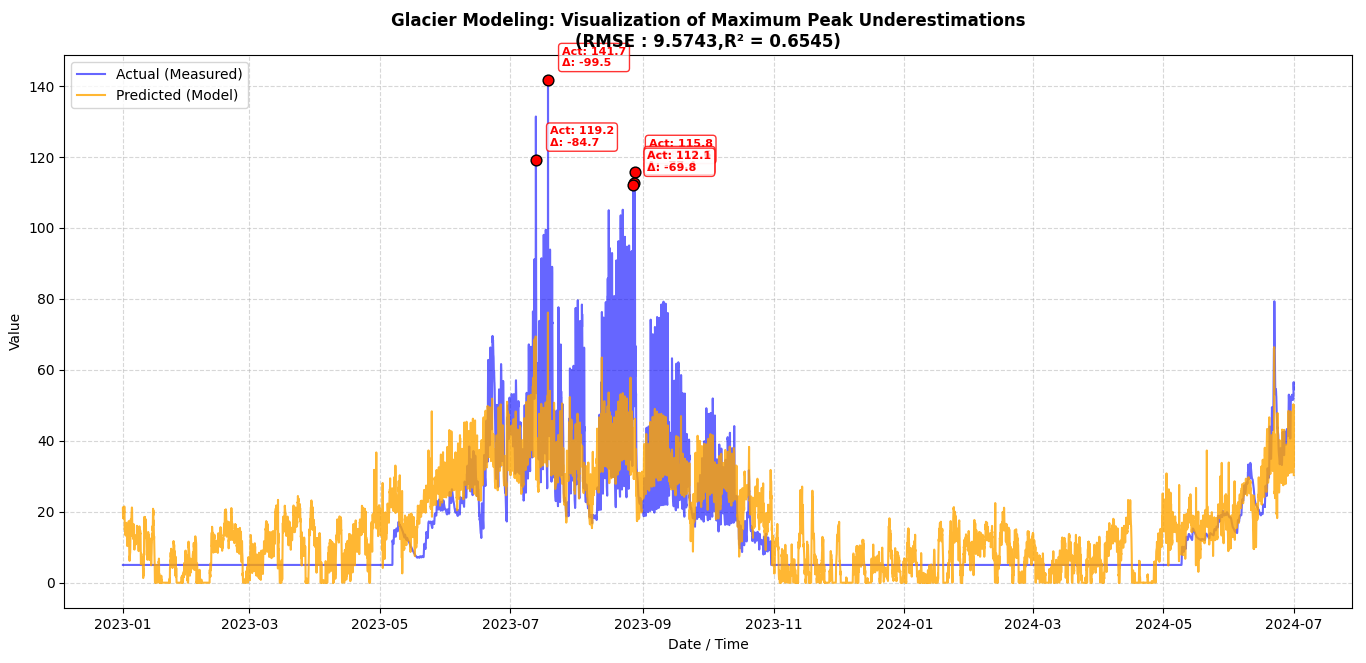
\includegraphics[width=\linewidth]{plots_H/WL_FE_plain_detail.png}
    \caption{Water level: Test period, plain data}
\end{figure}

Results with all additional features.
\begin{figure}[H]
    \centering
    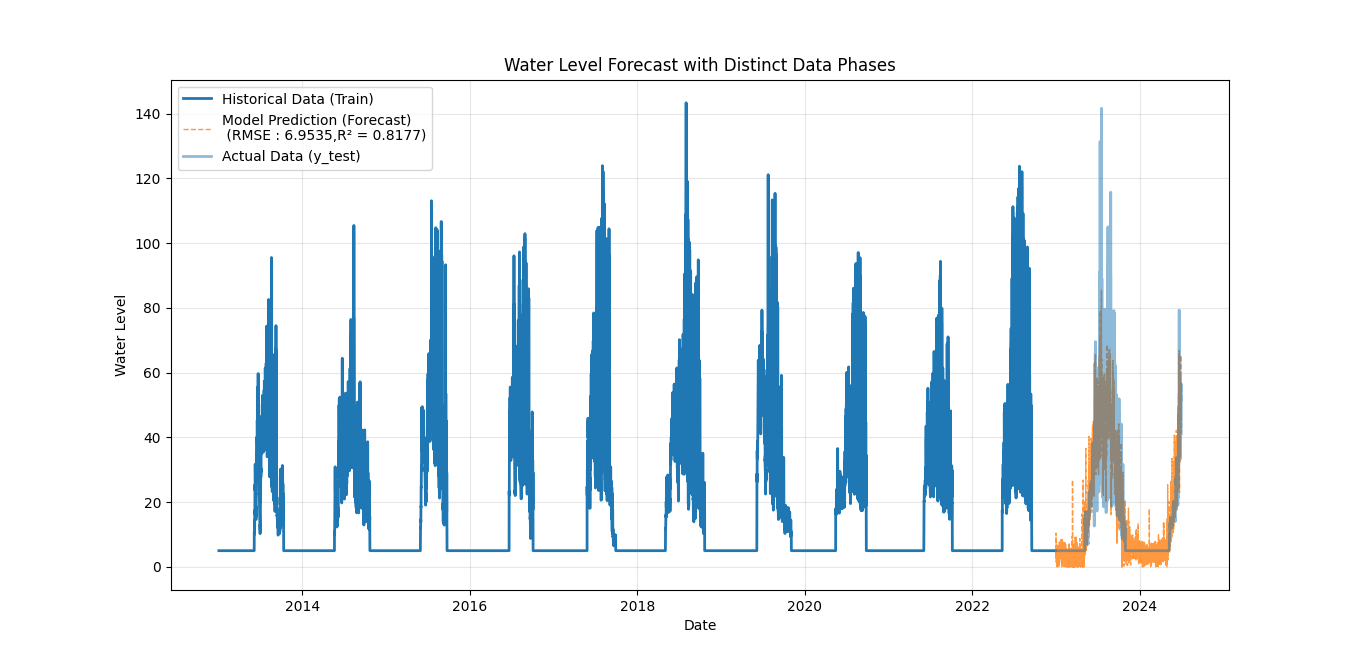
\includegraphics[width=\linewidth]
    {plots_H/WL_FE_saisona_y_d_snowmem_Lag.png}
    \label{fig:placeholder}
   \caption{Water level: Test period, with complete FE data}
\end{figure}

\begin{figure}[H]
    \centering
    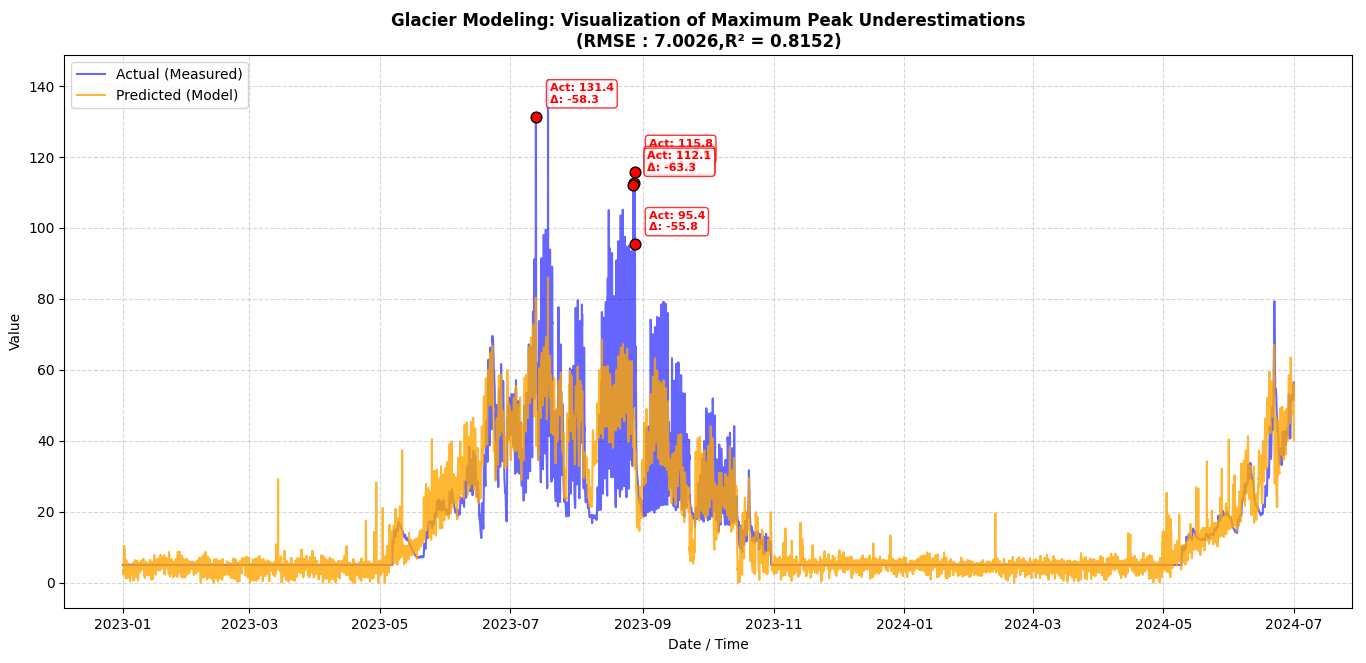
\includegraphics[width=\linewidth]{plots_H/WL_FE_saisona_y_d_snowmem_Lag_redv_detail.png}
    \caption{Water level: Test period, with complete FE data}
\end{figure}

\begin{table}[H]
    \centering
    \caption{Comparison of RMSE and $R^2$ metrics for different feature configurations, Test data}
    \label{tab:ml_metrics_comparison}
    \begin{tabular}{lll}
        \toprule
        \textbf{Configuration / Features} & {\textbf{RMSE}} & {\textbf{$R^2$}} \\
        \midrule
        Plain & 9.574 & 0.6545 \\
        Seasonality (d/y) & 8.498 & 0.7277 \\
        Seasonality (d/y) + Snow storage & 7.145 & 0.8076 \\
        Seasonality (d/y) + Snow storage + Lag features & 6.9535 & 0.8177 \\
        Seasonality (d/y) + Snow storage + Lag features + SK & 7.0228 & 0.8141 \\
        \bottomrule
    \end{tabular}
\end{table}

A continuous improvement can be seen when features detected in EDA and FE added to the model.

The error for the training data is higher than the error for the test data. This can be explained by the temporal asymmetry of the data split, which has a 5:1 ratio (a 10-year training period versus a 2-year test period). The much longer training timeframe inherently captures a higher density of meteorological anomalies, unrepresentative extreme events, and systemic noise that distort global fit metrics like the RMSE. Conversely, the shorter 2-year test period exhibits lower variance and fewer extreme shocks, allowing the seasonal and storage-based patterns learned during training to predict the unseen data with higher relative precision.

For comparison an alternative linear regression model is tested.
It evaluates the regression errors in a different way, which leads to different outcomes.

\paragraph*{GammaRegressor / Results}

For comparison an other linear ML model is applied to the problem. Difference (main): Residual do along with a gamma distribution.

This assumption has to be checked when deploy the model.

The results shown below are with complete FE generated features.

\begin{figure}[H]
    \centering
    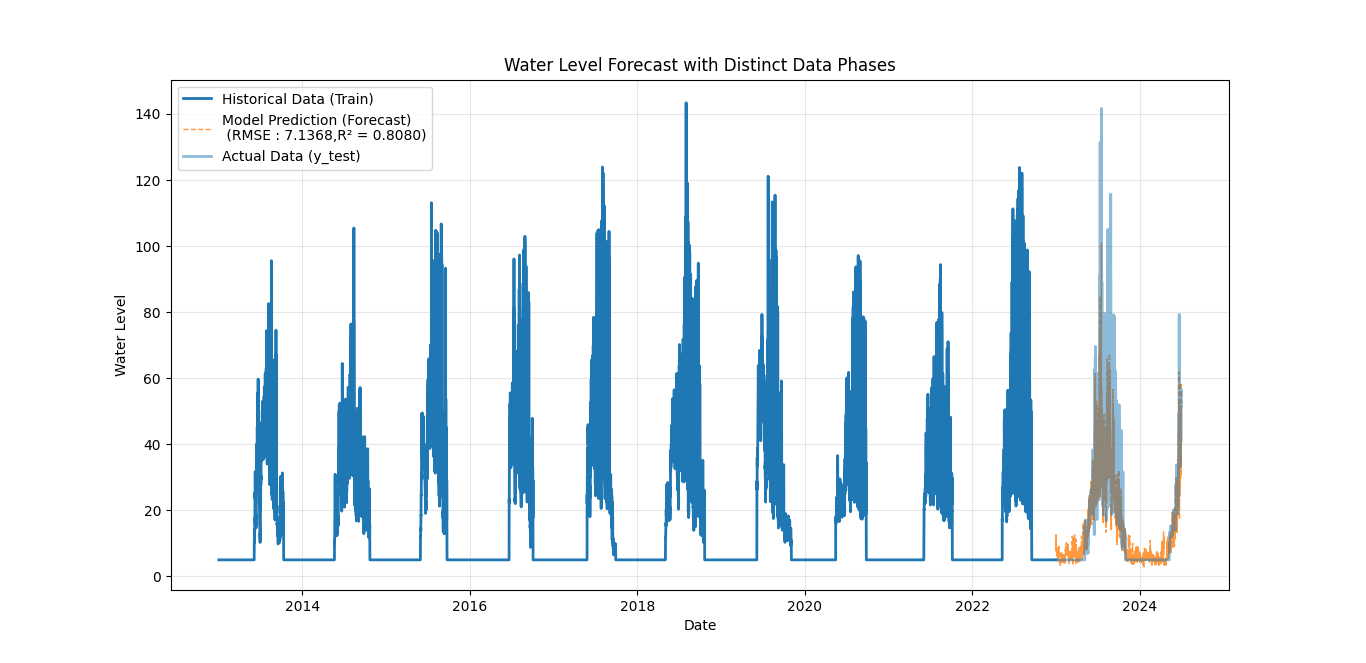
\includegraphics[width=\linewidth]{plots_H/Gamma_WL_FE_saisona_y_d_snowmem_Lag.png}
    \caption{Water level prediction}
\end{figure}

\begin{figure}[H]
    \centering
    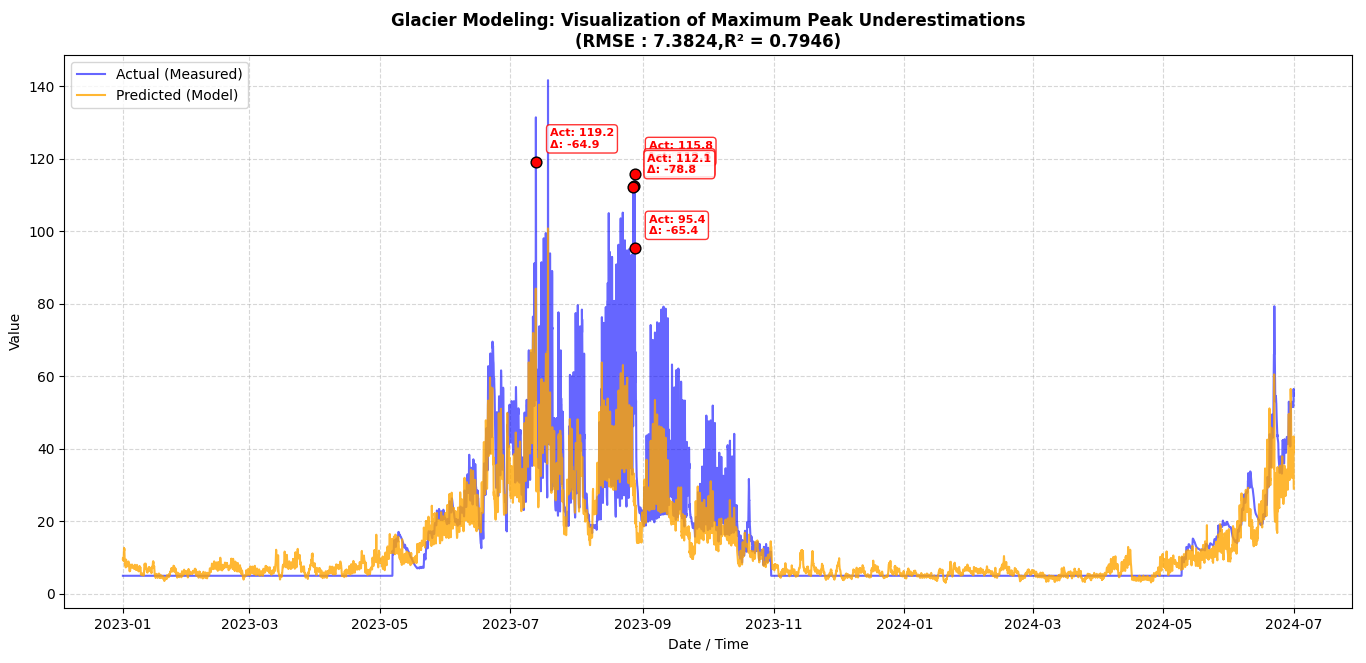
\includegraphics[width=\linewidth]{plots_H/Gamma_WL_FE_saisona_y_d_snowmem_Lag_detail.png}
    \caption{Water level prediction, Prediction detail}
\end{figure}

\begin{table}[H]
    \centering
    \caption{GammaRegressor RMSE and R2 metrics}
    \label{tab:modell_features}
    \begin{tabular}{lcc}
        \hline
        \textbf{Dataset Split} & \textbf{RMSE} & \textbf{\(R^2\)} \\ \hline
        Train                  & 9.8510        & 0.7187           \\
        Test                   & 7.3824        & 0.7946           \\ \hline
    \end{tabular}
\end{table}

\paragraph{Assumption check}

\begin{figure}[H]
    \centering
    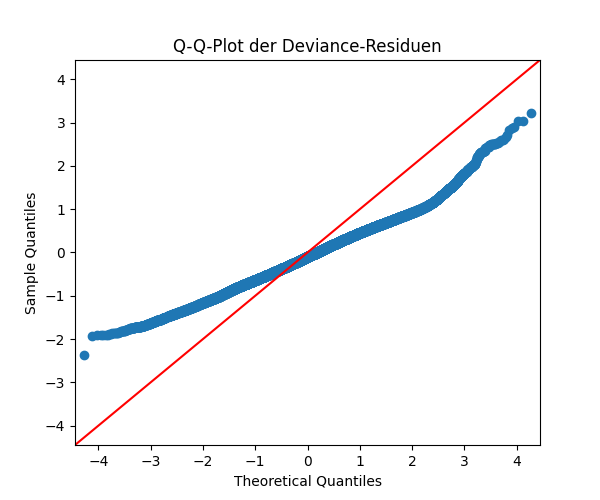
\includegraphics[width=\linewidth]{plots_H/Q-Q_Ti_comp.png}
    \caption{Water level prediction, Prediction detail}
\end{figure}

The Q-Q plot indicates a violation of the Gamma distribution assumption in the residuals. 
While this limits the interpretation of inferential statistics---such as $p$-values and 
confidence intervals---the predictive validity of the model remains unaffected. 
The high test $R^2$ of~0.79 and the low test RMSE of~7.38 demonstrate that, 
despite the violated theoretical variance structure, the model delivers a robust 
and highly accurate forecasting performance.

\subsubsection{Autoregressive models: Prophet and SAMIRAX}
\label{ssub:autoregressive_models}

Trained the models with a shortened DF because of computing time. Only synthetic features such as sinusoidal cycles for day and year were used.

\begin{description}

    \item[Prophet] \label{item:prophet}
    \FloatBarrier
    
    \begin{figure}[H]
        \centering
        \begin{subfigure}[b]{0.49\linewidth}
            \centering
            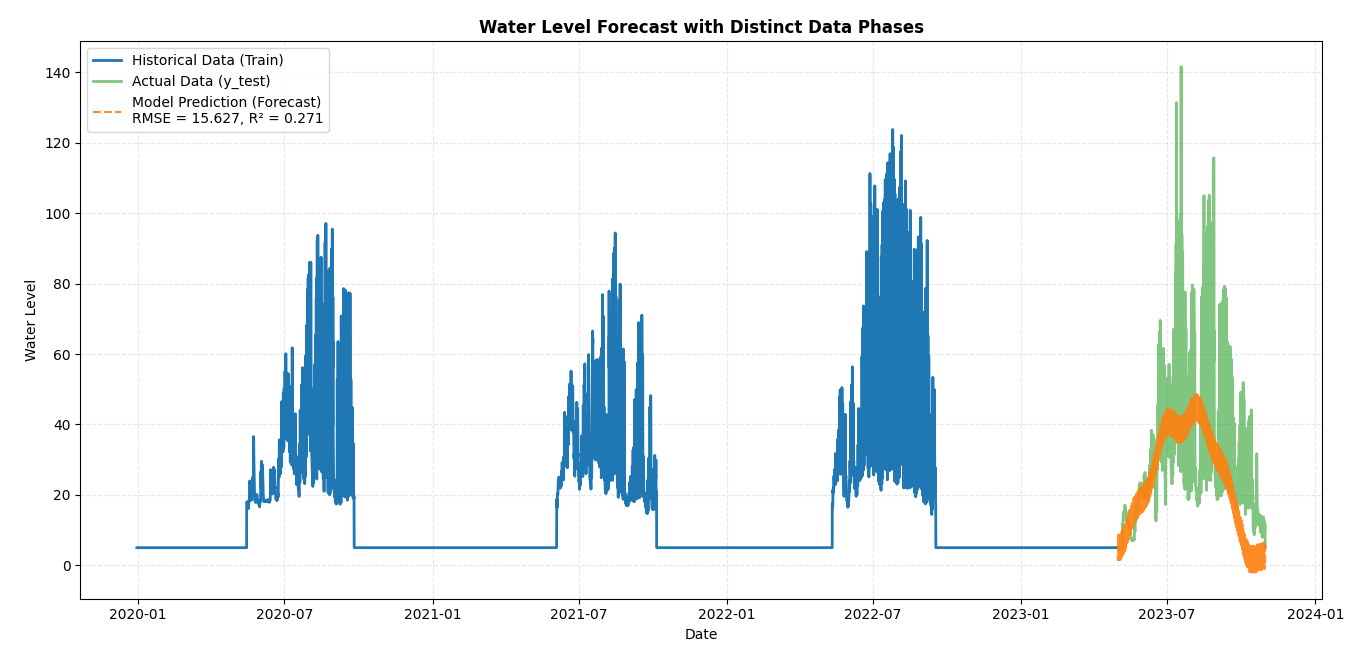
\includegraphics[width=\linewidth]{plots_H/Prohet_WL_plain.png}
            \caption{Overview}
            \label{fig:prophet_overview}
        \end{subfigure}
        \hfill
        \begin{subfigure}[b]{0.49\linewidth}
            \centering
            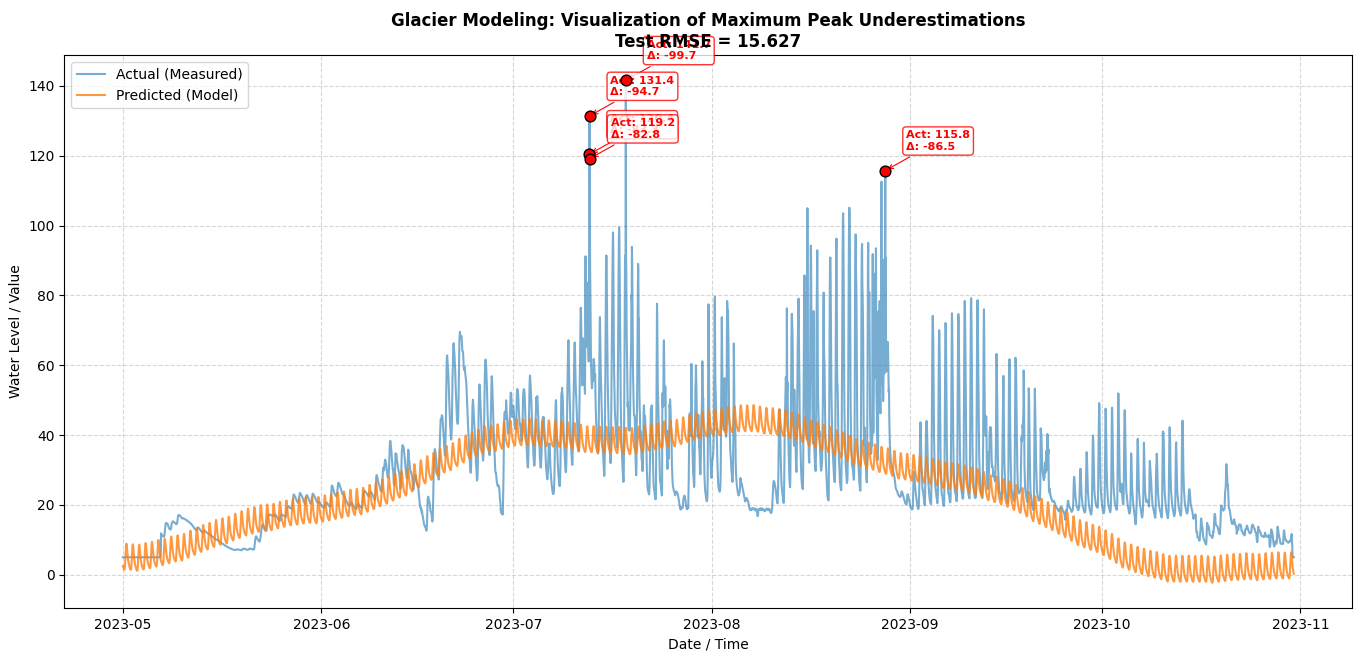
\includegraphics[width=\linewidth]{plots_H/Prohet_WL_plain_detail.png}
            \caption{Prediction detail}
            \label{fig:prophet_detail}
        \end{subfigure}
        \caption{Water level prediction using the Facebook Prophet model.}
        \label{fig:prophet_plots}
    \end{figure}
    
    \begin{table}[H]
        \centering
        \caption{Prophet Model Evaluation Metrics}
        \label{tab:prophet_evaluation1}
        \begin{tabular}{lcc}
            \toprule
            \textbf{Dataset Split} & \textbf{RMSE} & \textbf{\(R^2\)} \\ 
            \midrule
            Train                  & 8.853         & 0.733             \\
            Test                   & 15.627        & 0.271             \\ 
            \bottomrule
        \end{tabular}
    \end{table}
    
    Compared to the ML regression models the performance is worse. But in consideration of the pure forecast function and the complexity of the problem it's not that bad.
\newpage
    \item[SAMIRAX] \label{item:samirax}
    \FloatBarrier
    
    \begin{figure}[H]
        \centering
        \begin{subfigure}[b]{0.49\linewidth}
            \centering
            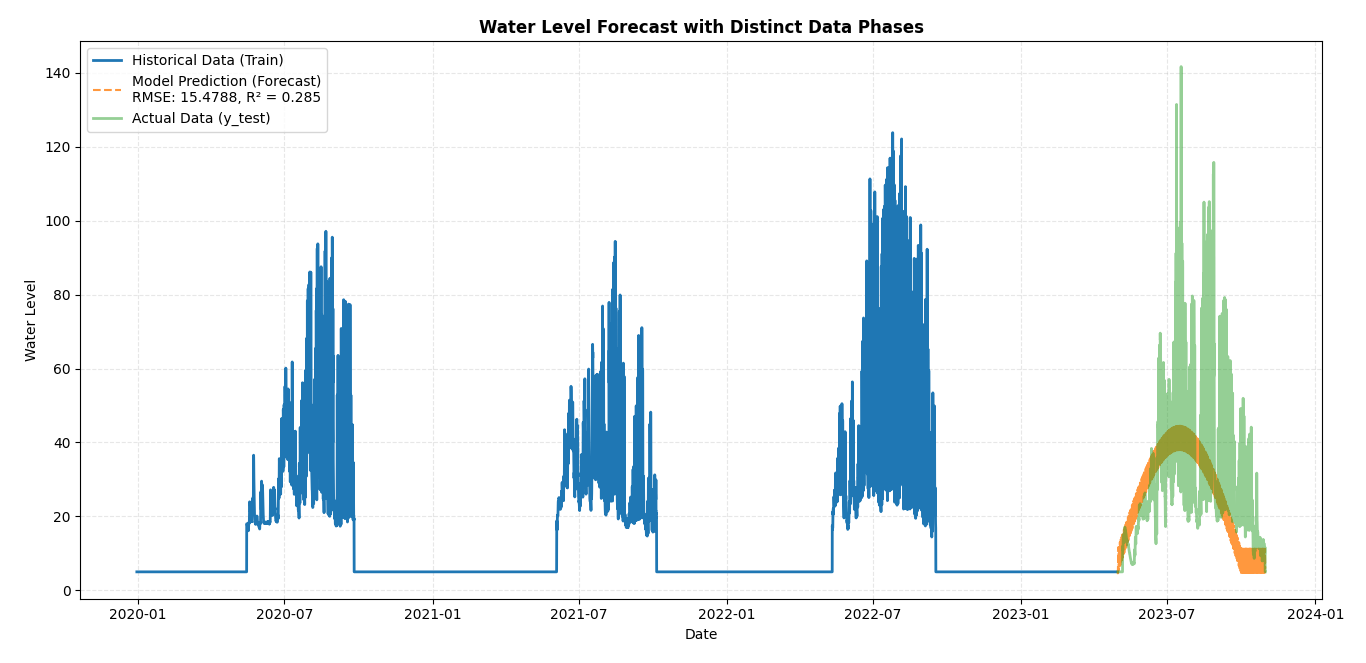
\includegraphics[width=\linewidth]{plots_H/SAMIRAX_WL_arti_exo_time_comp_opt.png}
            \caption{Overview}
            \label{fig:samirax_overview}
        \end{subfigure}
        \hfill
        \begin{subfigure}[b]{0.49\linewidth}
            \centering
            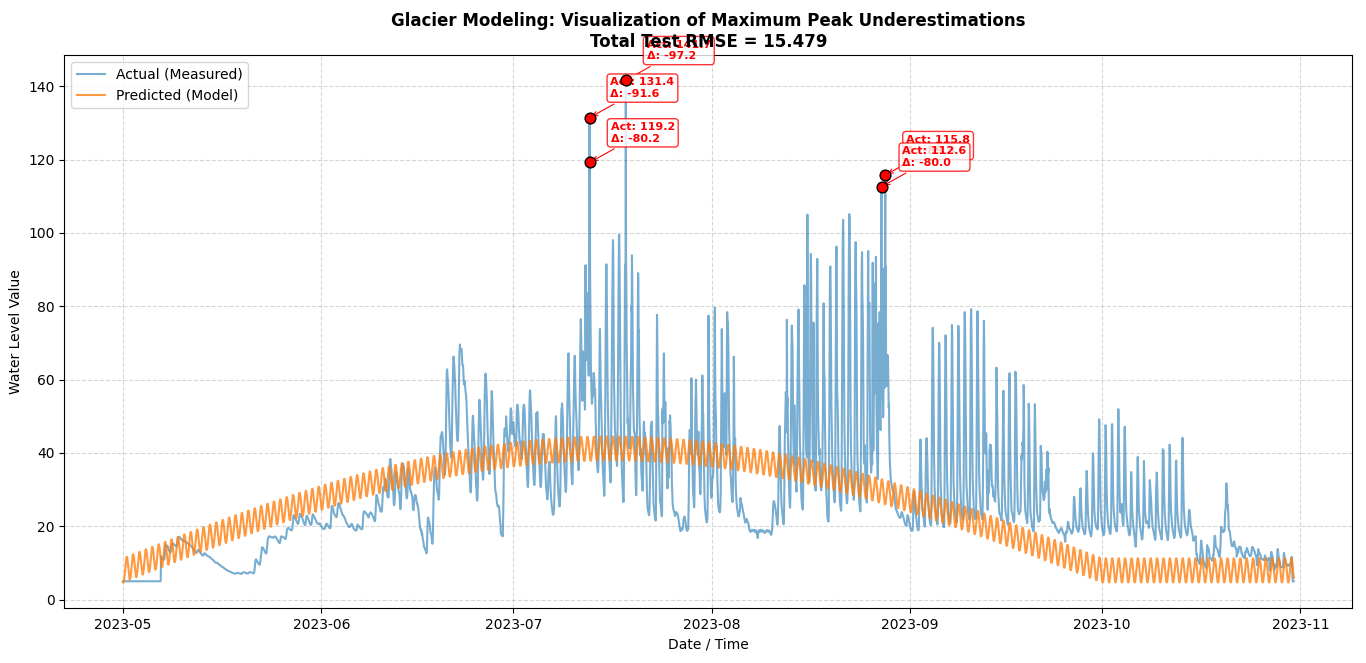
\includegraphics[width=\linewidth]{plots_H/SAMIRAX_WL_arti_exo_time_comp_opt_detail.png}
            \caption{Prediction detail}
            \label{fig:samirax_detail}
        \end{subfigure}
        \caption{Water level prediction using the SAMIRAX model (Historical Run).}
        \label{fig:samirax_plots}
    \end{figure}
    
    \begin{table}[H]
        \centering
        \caption{SAMIRAX Model Performance Metrics}
        \label{tab:samirax_metrics_hist}
        \begin{tabular}{lcc}
            \toprule
            \textbf{Dataset Split} & \textbf{RMSE} & \textbf{\(R^2\)} \\ 
            \midrule
            Test                   & 15.479        & 0.285             \\ 
            \bottomrule
        \end{tabular}
    \end{table}
    
    For the above analysis only the metrics for the test period are available. Which are comparable to the Prophet results. The reason is that the parameters for this result are not available anymore because of the poor documentation. The attempt to rebuild this status, is at the moment the rendering is due, not finished. For the results which are available so far, see below.
    
    \begin{figure}[H]
        \centering
        \begin{subfigure}[b]{0.49\linewidth}
            \centering
            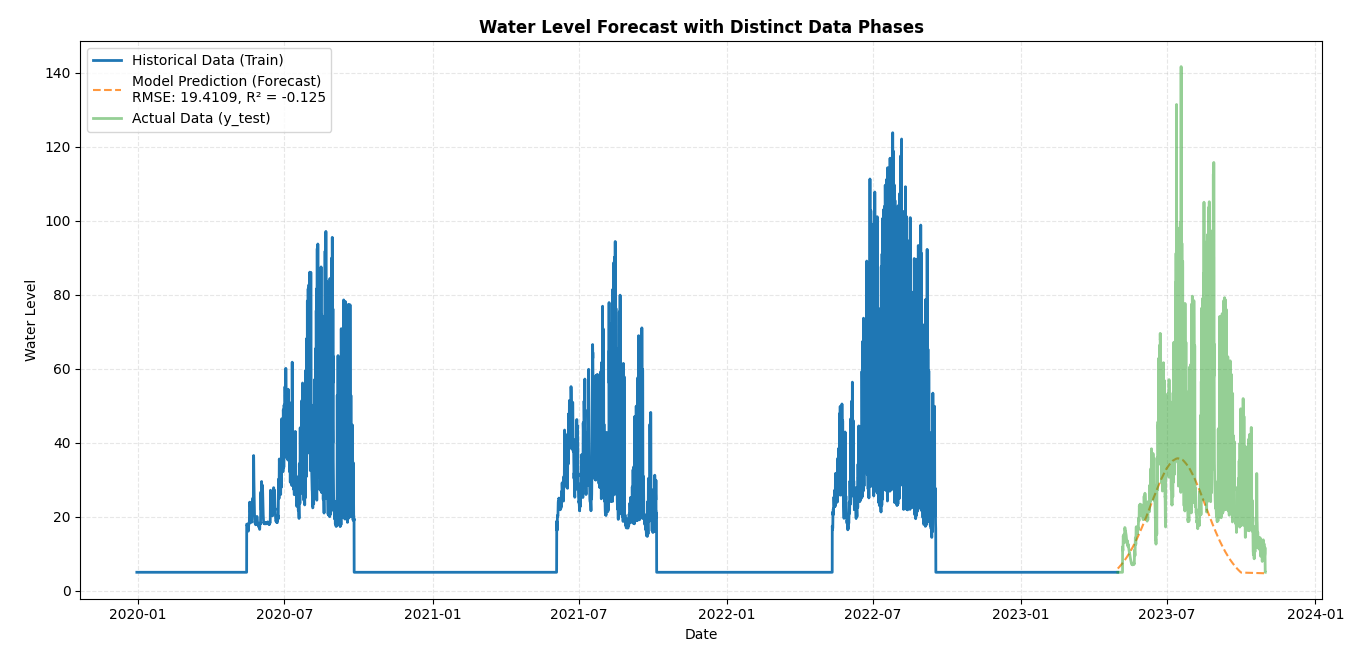
\includegraphics[width=\linewidth]{plots_H/SAMIRAX_WL_arti_exo_para_opt.png}
            \caption{Overview (Overfitted Run)}
            \label{fig:samirax_over_overview}
        \end{subfigure}
        \hfill
        \begin{subfigure}[b]{0.49\linewidth}
            \centering
            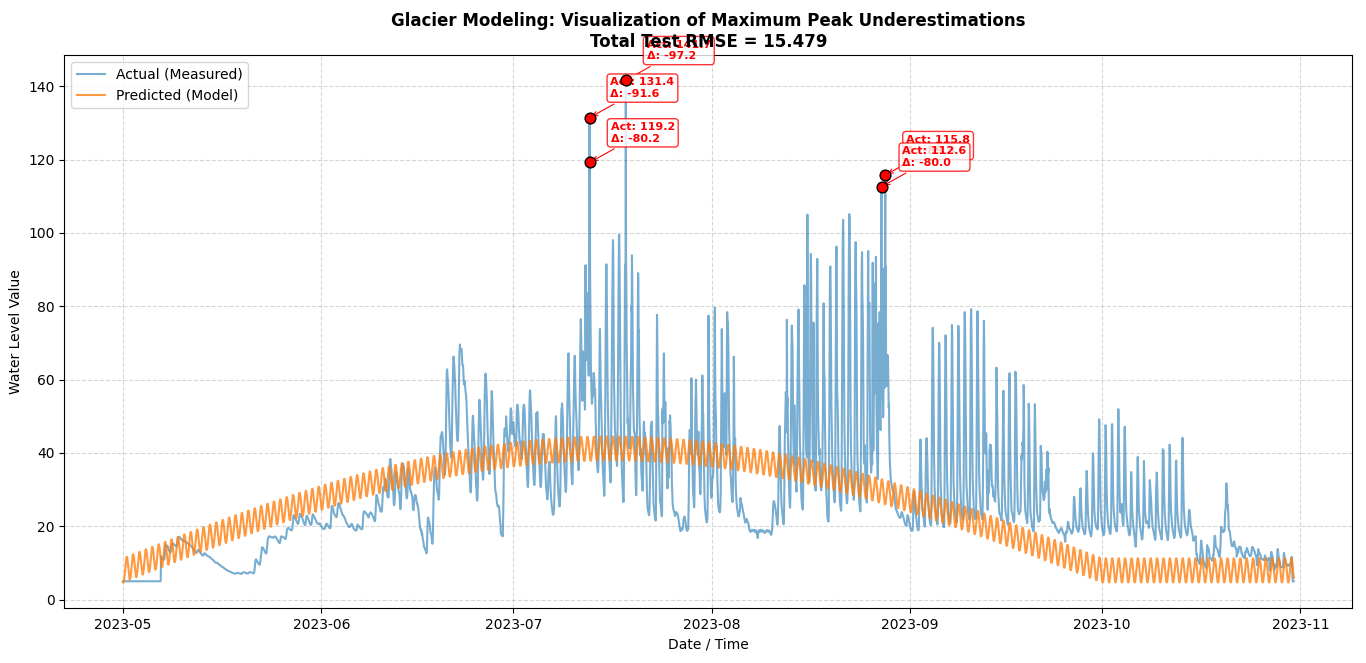
\includegraphics[width=\linewidth]{plots_H/SAMIRAX_WL_arti_exo_time_comp_opt_detail.png}
            \caption{Prediction detail (Overfitted Run)}
            \label{fig:samirax_over_detail}
        \end{subfigure}
        \caption{Water level prediction using the SAMIRAX model showing severe divergence.}
        \label{fig:samirax_plots_overfitted}
    \end{figure}
    
    \begin{table}[H]
        \centering
        \caption{SAMIRAX Model Evaluation Metrics (Overfitted Search)}
        \label{tab:samirax_metrics_overfitted}
        \begin{tabular}{lcc}
            \toprule
            \textbf{Dataset Split} & \textbf{RMSE} & \textbf{\(R^2\)} \\ 
            \midrule
            Train                  & 2.237         & 0.983             \\ 
            Test                   & 19.411        & -0.125            \\ 
            \bottomrule
        \end{tabular}
    \end{table}
    
    During the search for the lost parameters the results shown in figures above and shown in Table~\ref{tab:samirax_metrics_overfitted} occurred. This is an absolute overfitted model which led to poor results for the test period. 
    
    The negative coefficient of determination ($R^2 = -0.1250$) on the test dataset indicates that the model's out-of-sample predictions performed worse than a naive baseline model that simply predicts the mean of the actual observations. This negative goodness of fit suggests a severe structural divergence or accumulation of errors during the multi-step forecasting horizon.

\end{description}

\subsubsection{Lazypredictor classify best ML models}

For the search the data were accumulated on a daily basis to reduce computing time.

\begin{table}[H]
    \centering
    \caption{Performance evaluation of machine learning models using LazyPredictor}
    \label{tab:lazypredictor_results}
    \small % Verringert die Schriftgröße leicht, damit die Tabelle kompakt bleibt
    \begin{tabular}{lllll}
        \toprule
        \textbf{Model} & {\textbf{Adjusted $R^2$}} & {\textbf{$R^2$}} & {\textbf{RMSE}} & {\textbf{Time Taken (s)}} \\
        \midrule
        ExtraTreesRegressor & 0.7462 & 0.7474 & 9.2181 & 38.35 \\
        MLPRegressor & 0.7338 & 0.7351 & 9.4399 & 79.73 \\
        HistGradientBoostingRegressor & 0.7255 & 0.7268 & 9.5870 & 1.08 \\
        GradientBoostingRegressor & 0.7197 & 0.7211 & 9.6878 & 64.36 \\
        XGBRegressor & 0.7166 & 0.7180 & 9.7413 & 0.83 \\
        RandomForestRegressor & 0.6909 & 0.6924 & 10.1729 & 121.85 \\
        BaggingRegressor & 0.6754 & 0.6771 & 10.4239 & 15.47 \\
        PoissonRegressor & 0.6714 & 0.6730 & 10.4885 & 0.25 \\
        KNeighborsRegressor & 0.6673 & 0.6689 & 10.5545 & 1.02 \\
        ElasticNetCV & 0.6453 & 0.6470 & 10.8977 & 2.27 \\
        RidgeCV & 0.6449 & 0.6467 & 10.9033 & 0.58 \\
        BayesianRidge & 0.6449 & 0.6467 & 10.9033 & 0.29 \\
        Ridge & 0.6449 & 0.6467 & 10.9034 & 0.30 \\
        LassoLarsCV & 0.6449 & 0.6467 & 10.9034 & 0.72 \\
        LassoLarsIC & 0.6449 & 0.6467 & 10.9034 & 0.29 \\
        TransformedTargetRegressor & 0.6449 & 0.6467 & 10.9034 & 0.19 \\
        LinearRegression & 0.6449 & 0.6467 & 10.9034 & 0.20 \\
        SGDRegressor & 0.6441 & 0.6458 & 10.9162 & 1.18 \\
        LassoCV & 0.6437 & 0.6455 & 10.9219 & 1.82 \\
        LarsCV & 0.6320 & 0.6338 & 11.0995 & 0.74 \\
        Lars & 0.6268 & 0.6287 & 11.1771 & 0.19 \\
        OrthogonalMatchingPursuitCV & 0.6188 & 0.6207 & 11.2965 & 0.40 \\
        HuberRegressor & 0.6135 & 0.6154 & 11.3755 & 2.27 \\
        ElasticNet & 0.6059 & 0.6079 & 11.4863 & 0.22 \\
        LinearSVR & 0.6020 & 0.6040 & 11.5427 & 10.73 \\
        Lasso & 0.5960 & 0.5980 & 11.6299 & 0.21 \\
        LassoLars & 0.5960 & 0.5980 & 11.6301 & 0.15 \\
        GammaRegressor & 0.5959 & 0.5980 & 11.6306 & 1.72 \\
        TweedieRegressor & 0.5890 & 0.5910 & 11.7304 & 0.16 \\
        OrthogonalMatchingPursuit & 0.5562 & 0.5584 & 12.1888 & 0.15 \\
        ExtraTreeRegressor & 0.5108 & 0.5132 & 12.7975 & 0.55 \\
        AdaBoostRegressor & 0.5088 & 0.5112 & 12.8241 & 21.01 \\
        DecisionTreeRegressor & 0.4694 & 0.4720 & 13.3279 & 2.88 \\
        PassiveAggressiveRegressor & 0.4031 & 0.4060 & 14.1367 & 0.38 \\
        RANSACRegressor & -0.0470 & -0.0418 & 18.7222 & 0.75 \\
        DummyRegressor & -0.5534 & -0.5457 & 22.8048 & 0.13 \\
        QuantileRegressor & -1.8122 & -1.7981 & 30.6832 & 149.97 \\
        \bottomrule
    \end{tabular}
\end{table}

\paragraph{Summary of Machine Learning Model Evaluation*}
\label{sec:ml_summary}
A benchmarking analysis was conducted using \texttt{LazyPredictor} to evaluate 37 machine learning models on a meteorological and hydrological dataset. The objective was to predict water levels or discharge values based on feature engineering configurations including seasonality, snow storage, and lag variables.

The evaluation yielded the following key insights:
\begin{itemize}
    \item \textbf{Dominance of Ensemble Tree-Based Models:} Tree-based ensemble methods consistently outperformed classical linear models. The \texttt{ExtraTreesRegressor} achieved the highest predictive accuracy with an adjusted $R^2$ of $0.8364$ and the lowest Root Mean Squared Error ($\text{RMSE} = 7.8216$). 
    \item \textbf{Performance vs. Efficiency Trade-off:} While \texttt{ExtraTreesRegressor} and \texttt{MLPRegressor} provided top-tier accuracy, they required significant computational budgets ($28.00$\,s and $62.80$\,s, respectively). In contrast, histogram-based gradient boosting (\texttt{HistGradientBoostingRegressor}) achieved a highly competitive adjusted $R^2$ of $0.8245$ in a fraction of the time ($1.00$\,s), offering the optimal balance for real-time production deployment.
    \item \textbf{Failure of Linear Approaches:} Standard linear baselines (e.g., \texttt{Linear Regression}, \texttt{Ridge}) stalled at an adjusted $R^2$ of $0.7745$. These models are mathematically constrained to straight-line approximations and failed to capture the non-linear, multi-scale dynamics inherent in ecological systems.
\end{itemize}

\noindent Mathematically, the superior performance of tree-based structures in this environmental context is driven by three distinct data characteristics:
\begin{enumerate}
    \item \textbf{Non-Linearity:} Physical processes (such as the relationship between temperature and evaporation) scale non-linearly.
    \item \textbf{Feature Interactions:} Environmental triggers are coupled; for example, heavy rainfall creates severe runoff events only when combined with high initial soil moisture saturation or rapid snowmelt.
    \item \textbf{Threshold Effects:} Hydrological states change abruptly at distinct physical tipping points, such as freezing or melting thresholds ($0^\circ\text{C}$), which decision trees segment natively via recursive binary splits.
\end{enumerate}

Because of the performance v. efficiency trade off the HbGBR was chosen as reference ML model for this approach.

The Histogram-based Gradient Boosting Regressor is an advanced, highly scalable ensemble learning algorithm based on LightGBM. It optimizes the classical gradient boosting framework by binning continuous features into discrete histograms. This structural modification drastically accelerates the training process and reduces memory consumption while maintaining non-linear predictive power.

\subsubsection{Results for HbGBR}

The results shown are generated with all FE generated features.\\

\begin{figure}[H]
    \centering
    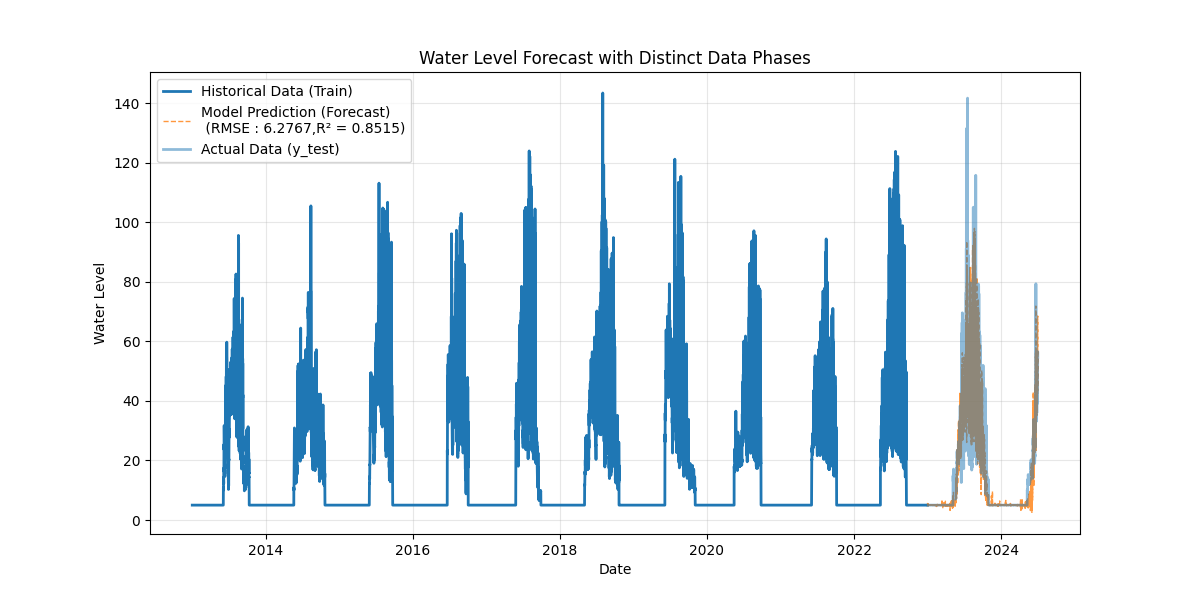
\includegraphics[width=\linewidth]{plots_H/HGBR_WL_FE_saison_snowmem_lag_Ti_comp.png}
    \caption{Water level prediction}
\end{figure}

\begin{figure}[H]
    \centering
    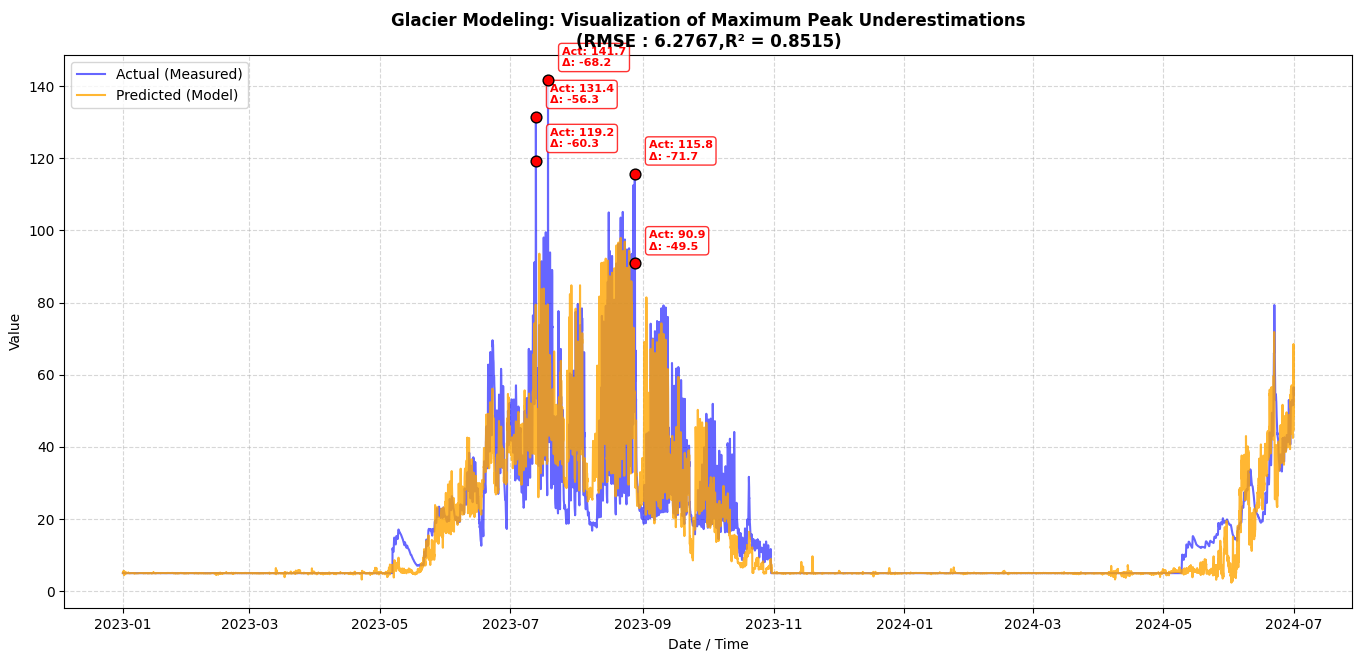
\includegraphics[width=\linewidth]{plots_H/HGBR_WL_FE_saison_snowmem_lag_Ti_comp_detail.png}
    \caption{Water level prediction, Prediction detail}
\end{figure}

\begin{table}[H]
    \centering
    \caption{Performance metrics for HbGB Train- and Test data}
    \label{tab:model_evaluation}
        \begin{tabular}{lcc}
        \hline
        \textbf{Metric} & \textbf{Train data (Train)} & \textbf{Test data (Test)} \\ \hline
        RMSE            & 6,2767                          & 4,0834                    \\
        $R^2$-Score     & 0,9517                          & 0,8515                    \\ \hline
    \end{tabular}
\end{table}

The HistGradientBoostingRegressor (HbGBR) achieved an outstanding performance, 
yielding a test coefficient of determination ($R^2$) of~0.8515 and a low test RMSE of~4.0834. This signifies a massive improvement over the other approaches. 

\subsection{Model Application of Deep Learning Models}
For setting up a Deep Learning Model the input data has to have a defined format. In this case the procedure of supplying the time series data for a Deep Learning Model led to the definition of a CustomDatasets in Pytorch. This CustomDataset creates chunks of the dataset with a given length of time (time span) that can be any consecutive chunk of the data with the given length. Although it is computationally expensive a model output is calculated for a time period by averaging all model outputs with the given length of time that are chunks of the data for that time period. The mean absolute error (mae) or the root mean squared error (rmse) can be calculated on the test data to evaluate the model. As loss function the mean absolute error (torch.nn.L1Loss) is used for validation and testing. The root mean squared error is computed to enable comparison with the Machine Learning Models.

The models are trained on two versions of input data. The first version comprises the longer time period of the measurements of Pegelstation Meteorologie and the water level from 2013-01-01 00:02:30 to 2024-07-31 18:17:30 and is called model\_PM\_*. The second version comprises all measurement data from 2015-07-22 11:57:30 to 2024-07-31 18:17:30 and is called model\_all\_*. The scripts for training were ported to www.kaggle.com to be able to use their computation power. The first results can be found in the following table.

\begin{table}[H]
\begin{tabular}{llll}
model name & mae & rmse & time span \\
\hline
model\_PM\_0 & 8.73 & 10.74 & 1 day \\
model\_all\_0 & 6.7 & 9.2 & 1 day \\
model\_pm\_1 & 5.87 & 8.41 & 7 days \\
model\_all\_1 & 6.49 & 9.38 & 7 days \\
\end{tabular}
\end{table}

\paragraph{model\_PM\_0, mae: 8.73, rmse: 10.74, time span: 1 day}

``model\_PM\_0'' (see figure \ref{fig:model_PM_0}) was the first try with only data from the Pegelstation Meteorologie, with a time span of 1 day and with small kernel sizes for the convolutional layers.

\begin{scriptsize}
\begin{verbatim}
Sequential(
  (0): Conv2d(1, 2, kernel_size=(3, 1), stride=(1, 1))
  (1): ReLU()
  (2): MaxPool2d(kernel_size=(4, 1), stride=(4, 1), padding=0, dilation=1, ceil_mode=False)
  (3): Conv2d(2, 4, kernel_size=(7, 1), stride=(1, 1))
  (4): ReLU()
  (5): MaxPool2d(kernel_size=(4, 1), stride=(4, 1), padding=0, dilation=1, ceil_mode=False)
  (6): Flatten(start_dim=1, end_dim=-1)
  (7): Linear(in_features=768, out_features=288, bias=True)
\end{verbatim}
\begin{verbatim}
==========================================================================================
Layer (type:depth-idx)                   Output Shape              Param #
==========================================================================================
Conv2d: 1-1                            [-1, 2, 286, 12]          8
ReLU: 1-2                              [-1, 2, 286, 12]          --
MaxPool2d: 1-3                         [-1, 2, 71, 12]           --
Conv2d: 1-4                            [-1, 4, 65, 12]           60
ReLU: 1-5                              [-1, 4, 65, 12]           --
MaxPool2d: 1-6                         [-1, 4, 16, 12]           --
Flatten: 1-7                           [-1, 768]                 --
Linear: 1-8                            [-1, 288]                 221,472
==========================================================================================
\end{verbatim}
\end{scriptsize}
\begin{figure}[h]
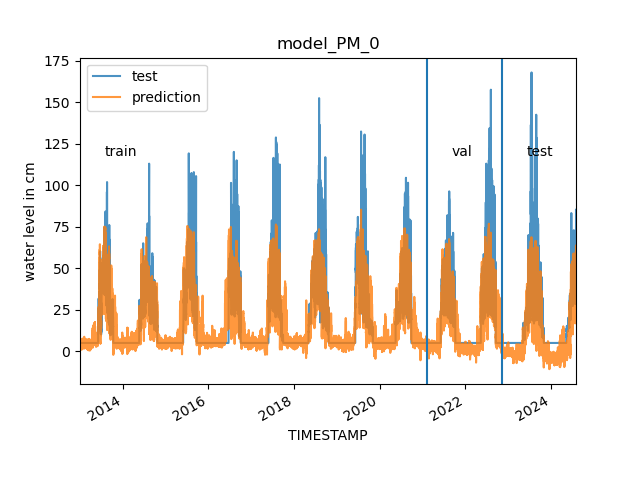
\includegraphics[width=0.75\textwidth]{plots_T/model_PM_0_result.png}
\caption{Graphical presentation of model\_PM\_0}
\label{fig:model_PM_0}
\end{figure}

\paragraph{model\_all\_0, mae: 6.7, rmse: 9.2, time span: 1 day}

``model\_all\_0'' (see figure \ref{fig:model_all_0}) is about the same as ``model\_PM\_0'' with a time span of 1 day and small kernel sizes for the convolutional layers but with an overall shorter time period of measurements but additional measurements from Schwarzkögele.

\begin{scriptsize}
\begin{verbatim}
Sequential(
  (0): Conv2d(1, 2, kernel_size=(3, 1), stride=(1, 1))
  (1): ReLU()
  (2): MaxPool2d(kernel_size=(4, 1), stride=(4, 1), padding=0, dilation=1, ceil_mode=False)
  (3): Conv2d(2, 4, kernel_size=(7, 1), stride=(1, 1))
  (4): ReLU()
  (5): MaxPool2d(kernel_size=(4, 1), stride=(4, 1), padding=0, dilation=1, ceil_mode=False)
  (6): Flatten(start_dim=1, end_dim=-1)
  (7): Linear(in_features=960, out_features=288, bias=True)
)
\end{verbatim}
\begin{verbatim}
==========================================================================================
Layer (type:depth-idx)                   Output Shape              Param #
==========================================================================================
Conv2d: 1-1                            [-1, 2, 286, 15]          8
ReLU: 1-2                              [-1, 2, 286, 15]          --
MaxPool2d: 1-3                         [-1, 2, 71, 15]           --
Conv2d: 1-4                            [-1, 4, 65, 15]           60
ReLU: 1-5                              [-1, 4, 65, 15]           --
MaxPool2d: 1-6                         [-1, 4, 16, 15]           --
Flatten: 1-7                           [-1, 960]                 --
Linear: 1-8                            [-1, 288]                 276,768
==========================================================================================
\end{verbatim}
\end{scriptsize}
\begin{figure}[h]
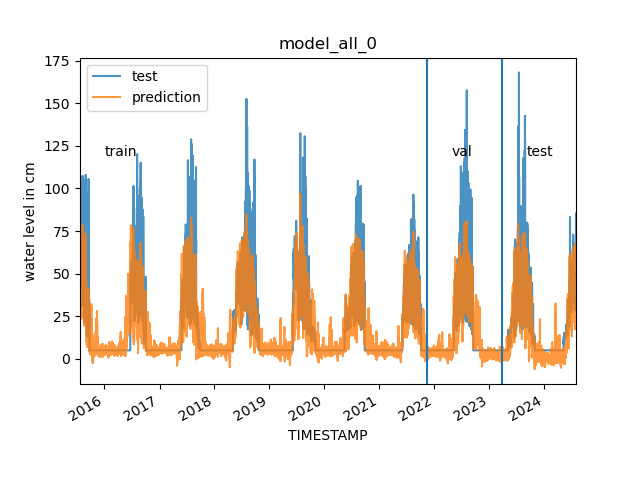
\includegraphics[width=0.75\textwidth]{plots_T/model_all_0_result.png}
\caption{Graphical presentation of model\_all\_0}
\label{fig:model_all_0}
\end{figure}

\paragraph{model\_PM\_1, mae: 5.87, rmse: 8.41, time span: 7 days}

``model\_PM\_1'' (see figure \ref{fig:model_pm_1}) has a longer time span than ``model\_PM\_0'' of 7 days and following that larger kernel sizes of the convolutional layers.

\begin{scriptsize}
\begin{verbatim}
Sequential(
  (0): Conv2d(1, 2, kernel_size=(13, 1), stride=(1, 1))
  (1): ReLU()
  (2): MaxPool2d(kernel_size=(4, 1), stride=(4, 1), padding=0, dilation=1, ceil_mode=False)
  (3): Conv2d(2, 4, kernel_size=(72, 1), stride=(1, 1))
  (4): ReLU()
  (5): MaxPool2d(kernel_size=(4, 1), stride=(4, 1), padding=0, dilation=1, ceil_mode=False)
  (6): Flatten(start_dim=1, end_dim=-1)
  (7): Linear(in_features=5136, out_features=2016, bias=True)
)
\end{verbatim}
\begin{verbatim}
==========================================================================================
Layer (type:depth-idx)                   Output Shape              Param #
==========================================================================================
Conv2d: 1-1                            [-1, 2, 2004, 12]         28
ReLU: 1-2                              [-1, 2, 2004, 12]         --
MaxPool2d: 1-3                         [-1, 2, 501, 12]          --
Conv2d: 1-4                            [-1, 4, 430, 12]          580
ReLU: 1-5                              [-1, 4, 430, 12]          --
MaxPool2d: 1-6                         [-1, 4, 107, 12]          --
Flatten: 1-7                           [-1, 5136]                --
Linear: 1-8                            [-1, 2016]                10,356,192
==========================================================================================
\end{verbatim}
\end{scriptsize}
\begin{figure}[h]
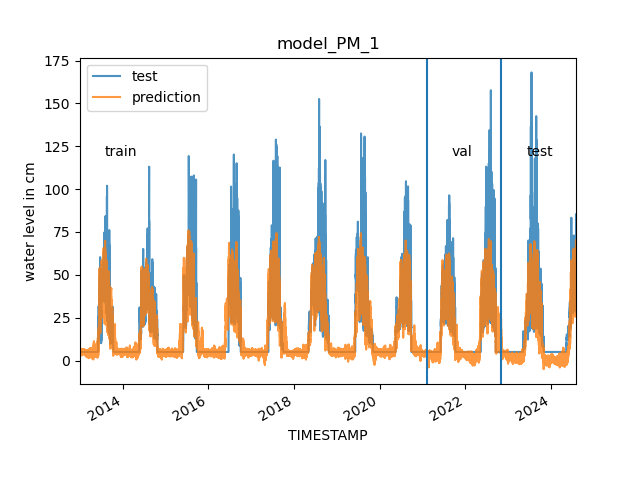
\includegraphics[width=0.75\textwidth]{plots_T/model_PM_1_result.png}
\caption{Graphical presentation of model\_PM\_1}
\label{fig:model_pm_1}
\end{figure}

\paragraph{model\_all\_1, mae: 6.49, rmse: 9.38, time span: 7 days}

``model\_all\_1'' (see figure \ref{fig:model_all_1}) has corresponding to ``model\_PM\_1'' a longer time span than ``model\_all\_0'' of 7 days and following that larger kernel sizes of the convolutional layers like ``model\_PM\_1''.

\begin{scriptsize}
\begin{verbatim}
Sequential(
  (0): Conv2d(1, 2, kernel_size=(13, 1), stride=(1, 1))
  (1): ReLU()
  (2): MaxPool2d(kernel_size=(4, 1), stride=(4, 1), padding=0, dilation=1, ceil_mode=False)
  (3): Conv2d(2, 4, kernel_size=(72, 1), stride=(1, 1))
  (4): ReLU()
  (5): MaxPool2d(kernel_size=(4, 1), stride=(4, 1), padding=0, dilation=1, ceil_mode=False)
  (6): Flatten(start_dim=1, end_dim=-1)
  (7): Linear(in_features=6420, out_features=2016, bias=True)
)
\end{verbatim}
\begin{verbatim}
==========================================================================================
Layer (type:depth-idx)                   Output Shape              Param #
==========================================================================================
Conv2d: 1-1                            [-1, 2, 2004, 15]         28
ReLU: 1-2                              [-1, 2, 2004, 15]         --
MaxPool2d: 1-3                         [-1, 2, 501, 15]          --
Conv2d: 1-4                            [-1, 4, 430, 15]          580
ReLU: 1-5                              [-1, 4, 430, 15]          --
MaxPool2d: 1-6                         [-1, 4, 107, 15]          --
Flatten: 1-7                           [-1, 6420]                --
Linear: 1-8                            [-1, 2016]                12,944,736
==========================================================================================
\end{verbatim}
\end{scriptsize}
\begin{figure}[h]
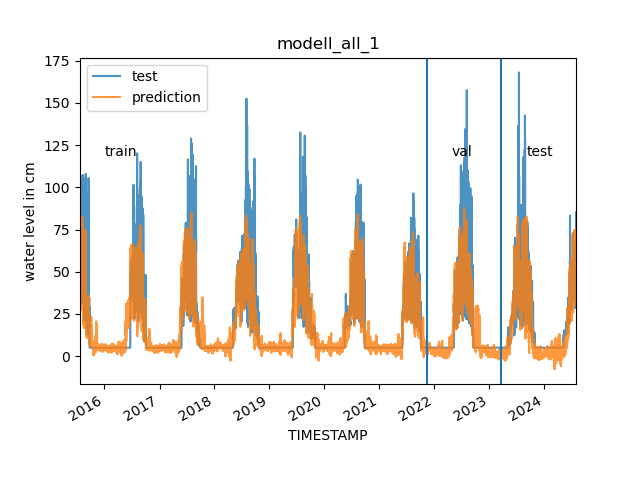
\includegraphics[width=0.75\textwidth]{plots_T/model_all_1_result.png}
\caption{Graphical presentation of model\_all\_1}
\label{fig:model_all_1}
\end{figure}

\section{Conclusion}
\subsection{Conclusion on Machine Learning Models}

The model evaluation demonstrates a clear superiority of non-linear machine learning 
architectures over traditional linear approaches for the glacier dataset. The 
HistGradientBoostingRegressor (HbGBR) emerged as the best-performing model, achieving 
the highest coefficient of determination ($R^2 = 0.8515$) and the lowest prediction 
error ($\text{RMSE} = 4.0834$) on the unseen test data. 

While the baseline Linear Regression delivered a robust fit ($R^2 = 0.8141$, $\text{RMSE} = 7.0228$), 
the Gamma Regressor fell slightly short ($R^2 = 0.7946$, $\text{RMSE} = 7.3824$). 
The significant performance leap generated by the HbGBR confirms that the underlying 
hydrological and meteorological processes contain complex, high-order feature 
interactions—such as the non-linear relationship between seasonal temperature arcs 
and delayed snow storage release—which linear frameworks fail to fully resolve.

\begin{table}[H]
    \centering
    \caption{Comparison of Machine Learning Models across Dataset Splits}
    \label{tab:ml_model_comparison}
    \begin{tabular}{lcccc}
        \hline
        \textbf{Model / Architecture} & \textbf{RMSE (Train)} & \textbf{RMSE (Test)} & \textbf{\(R^2\) (Train)} & \textbf{\(R^2\) (Test)} \\ \hline
        Linear Regression (OLS)       & --                    & 7.0228               & --                       & 0.8141                  \\
        Gamma Regressor (GLM)         & 9.8510                & 7.3824               & 0.7187                   & 0.7946                  \\
        HbGBR (Gradient Boosting)     & 6.2767                & 4.0834               & 0.9517                   & 0.8515                  \\ \hline
    \end{tabular}
\end{table}

\subsubsection{Dynamic behavior of the models}

A visual inspection of the hydrograph predictions (see Figures with detail plots) 
further substantiates the statistical superiority of the HbGBR. Traditional linear 
models inherently suffer from peak attenuation, systematically underestimating the 
maximum discharge spikes during the peak melt season (July--September 2023). 
In contrast, the HbGBR demonstrates a highly dynamic response, capturing the absolute 
magnitude of these extreme events with significantly lower deviations, although the lokal ($\Delta$) are smaller in the linear regression model, ca. -71cm (HbGBR) to -63cm (LR). Respectively, ca. -71cm (HbGBR) to -68cm (GammaR) what fits to the overall impression.

Furthermore, the HbGBR effectively filters out high-frequency noise during the 
winter baseline periods (November 2023 to May 2024), where it accurately models the 
near-zero plateau, whereas the linear framework introduces artificial volatility.\\

\subsubsection{Autocorrelation Models (Prophet and SARIMAX)}

The evaluation reveals a sharp performance dichotomy between tabular machine learning 
architectures and traditional time-series frameworks. Both the additive Facebook Prophet 
model and the autoregressive SARIMAX framework yielded poor out-of-sample performance, 
with coefficients of determination ($R^2$) hovering around~0.25. 

This localized failure is a well-documented constraint of multi-step-ahead forecasting 
on high-frequency (hourly) datasets. Because classical auto regressive models must iteratively 
rely on their own historical predictions over a prolonged 6-month test horizon, 
stochastic errors propagate exponentially, resulting in severe baseline drift.

Furthermore, the physical dynamics governing glacier ablation exhibit non-linear 
threshold interactions---such as the sudden release of meltwater when temperature markers 
intersect with depleted snow storage layers. While the ensemble-based 
HistGradientBoostingRegressor (HbGBR) can naturally segment and map these abrupt mathematical 
discontinuities (achieving a superior test $R^2$ of~0.8515), Prophet and SARIMAX are constrained by smooth, additive, or linear assumptions, rendering them incapable of 
resolving highly volatile discharge peaks.

\subsection{Conclusion on Deep Learning Models}

It was possible to get a Deep Learning Model running. The set up of the input data to the model was very difficult  but a solution could be found. The first results are only as good as a linear regression but there was no time for improvement of the first tries as the training of the models was very time consuming. There is very likely improvement on the data loading part and the training part possible which would lead to much lower computation times. With more time for the project more model architectures could have been be tried out to find an architecture that captures better the non-linearity of the variables.

\section{Outlook}

After gaining more experience on the set up of Deep Learning Models it should be possible to improve the existing first tries of Deep Learning Models. There exist physical models to model the discharge of a glacier stream which is deduced from the water level ([1] A. Lambrecht and C. Mayer, “The role of the cryosphere for runoff in a highly glacierised alpine catchment, an approach with a coupled model and in situ data,” Journal of Glaciology, vol. 70, p. e33, 2024. doi:10.1017/jog.2024.48). These models require a lot of different kinds of input data and are hard to operate. With a good Deep Learning Model found that can easier model aspects of a small earth system such as a glacier the principles of the model development could be applied to other small earth systems. This could help in modeling of earth system on smaller scales than it is possible at the moment.

\end{document}
